\documentclass[smallextended]{svjour3}
\smartqed
\usepackage[T1]{fontenc}
\usepackage[utf8]{inputenc}
\usepackage{lmodern,amsmath,amssymb,mathtools,microtype}
\usepackage{graphicx,booktabs,array,longtable,xurl}
\usepackage{tikz}
\usetikzlibrary{arrows.meta,calc,patterns}
\usepackage[colorlinks=true,allcolors=black,bookmarksnumbered=true]{hyperref}
% Mathematical Programming restricts the reference list to published/accepted
% work. These identifiers mention unpublished work directly in the text.
% Optional argument gives a locator in the explicitly identified version.
\makeatletter
\newcommand{\preprintcite}[2][]{%
  \@ifundefined{bfgspreprint@#2}%
    {\PackageError{bfgs-paper}{Unknown preprint key #2}{Define the verified source in preprint_references.tex.}}%
    {(\csname bfgspreprint@#2\endcsname\if\relax\detokenize{#1}\relax\else, #1\fi)}%
}
\@namedef{bfgspreprint@XW}{Xie and W\"achter, 2017 preprint,
  \href{https://arxiv.org/abs/1712.08571v1}{arXiv:1712.08571v1}}
\@namedef{bfgspreprint@DY}{Dyatlov, \emph{Notes on hyperbolic dynamics},
  2018 preprint, \href{https://arxiv.org/abs/1805.11660v1}{arXiv:1805.11660v1}}
\@namedef{bfgspreprint@LW}{Lewis and Wylie, 2019 preprint,
  \href{https://arxiv.org/abs/1907.11742}{arXiv:1907.11742}}
\@namedef{bfgspreprint@NEG_LO08}{Lewis and Overton,
  \href{https://cs.nyu.edu/overton/papers/pdffiles/bfgs_exactLS.pdf}{\emph{Behavior of BFGS with an Exact Line Search on Nonsmooth Examples}},
  2008 manuscript}
\@namedef{bfgspreprint@NEG_DIAO26}{Diao, 2026 preprint,
  \href{https://arxiv.org/abs/2609.09686v1}{arXiv:2609.09686v1}}
% This is a version pointer for LL, not a second canonical bibliography entry.
\@namedef{bfgspreprint@LL18}{Lewis and Liang, 2018 preprint,
  \href{https://arxiv.org/abs/1807.03134v1}{arXiv:1807.03134v1}}
% FND_JM25 is published in NeurIPS 2025 and is cited normally. This alias is
% available only when a locator specifically concerns its earlier version.
\@namedef{bfgspreprint@JM25v2}{Jin and Mokhtari, 2025 preprint version,
  \href{https://arxiv.org/abs/2507.00361v2}{arXiv:2507.00361v2}}
\makeatother

\newcommand{\R}{\mathbb R}
\newcommand{\norm}[1]{\lVert#1\rVert}
\DeclareMathOperator{\tr}{tr}
\DeclareMathOperator{\aff}{aff}
\DeclareMathOperator{\conv}{conv}
\DeclareMathOperator{\dist}{dist}
\DeclareMathOperator{\argmin}{argmin}
\setlength{\emergencystretch}{1.5em}
\allowdisplaybreaks[1]
\title{BFGS on Convex Nonsmooth Functions:\\Local Convergence and Failure}
\titlerunning{BFGS: local convergence and failure}
\author{}
\institute{}
\journalname{}
% Author-review layout: omit the editor's manuscript-number placeholder and
% the reserved empty author block. The class and body typography are unchanged.
\renewcommand{\makeheadbox}{}
\setlength{\headerboxheight}{0pt}
\date{Author-review edition, 12 September 2026}
\hypersetup{pdftitle={BFGS on Convex Nonsmooth Functions: Local Convergence and Failure},pdfsubject={Unmodified full BFGS; local convergence and deterministic failure},pdfkeywords={BFGS, convex nonsmooth optimization, local convergence, formal verification}}
\begin{document}
\maketitle
\begin{abstract}
We study unmodified full BFGS on finite convex nonsmooth objectives, with
Armijo--weak-Wolfe steps and actual gradients at differentiable accepted
iterates. The main contrast concerns local geometry. A finite polyhedral
partition near a unique minimizer, with locally Lipschitz gradient extensions
on its cells, gives a common local convergence basin for every positive
definite initial matrix. In contrast, a maximum of four globally convex
$C^{2,1}$ functions with uniformly bounded Hessians admits deterministic
nonstationary limits from starting points arbitrarily close to its unique
minimizer. A separate construction retains uniform strong convexity with
$C^{1,1}$ branches that lose second differentiability at the accumulation
point. All accepted and rejected queries in these examples are differentiable
and can remain arbitrarily close to the optimizer. The positive analysis
uses a reference-energy identity, a hierarchy of actual principal minors
of the full BFGS matrices, and reciprocal growth under bounded gradients
and vanishing predicted decreases. A transported comparison certificate
then relates this matrix budget to the objective's geometry. Neither the
positive analysis nor the counterexample construction presumes iterate
convergence or a matrix limit. Exact rational certificates, infinite
scaling inductions, and a reviewed Lean correspondence support the proofs;
the formal audit is distinguished from novelty and prose verification.
\keywords{BFGS \and convex nonsmooth optimization \and local convergence \and counterexample \and formal verification}
\subclass{90C30 \and 90C53 \and 49J52}
\end{abstract}
\section{Introduction and main results}\label{art:introduction}

Can ordinary BFGS converge locally on a convex objective whose gradients jump?
Regularity of the formulas defining the objective does not by itself settle
this question. We prove local convergence when a finite polyhedral arrangement
controls the nearby smooth pieces, and construct local failure when four smooth
convex formulas encode an accumulating sequence of bad switching configurations.
The distinction is between the geometry of switching and the regularity within
individual branches. It persists when all gradients queried by the algorithm
are ordinary derivatives.

Throughout, BFGS means the unmodified full inverse update. An infinite
\emph{admissible run} starts with any positive definite matrix, uses fixed
$0<c_1<c_2<1$, satisfies Armijo decrease and weak Wolfe curvature, and accepts
only differentiable points with nonzero gradients; the equations are given in
Definition~\ref{art:admissible}. This notion describes successful successive
line searches. It does not guarantee that every search ray contains a
differentiable acceptable point. The negative results instead verify every
decision of one specified unit-first doubling/bisection implementation.

The following theorem gives the main positive contrast. The local extensions
are defined on open sets, so smoothness at cell boundaries has a precise meaning.
\begin{theorem}[Local convergence on finite polyhedral cells]\label{art:polyhedral}
Let $n\ge1$ and let $F:\R^n\to\R$ be finite and convex, with a unique minimizer $x_*$.
Suppose an open neighborhood $U$ of $x_*$ is covered by finitely many closed
full-dimensional polyhedra $P_i$. For each $i$, suppose there is an open set
$V_i\supset U\cap P_i$ and a function $f_i\in C^{1,1}_{\rm loc}(V_i)$ such that
\[
 F(x)=f_i(x)\qquad(x\in U\cap P_i).
\]
Then there exists $\varepsilon>0$ such that every infinite full-BFGS run with
arbitrary $H_0\succ0$, differentiable accepted iterates, fixed
Armijo--weak-Wolfe constants $0<c_1<c_2<1$, and
$F(x_0)\le F(x_*)+\varepsilon$ satisfies
\[
 x_k\in U\quad(k\ge0),\qquad F(x_k)\to F(x_*),\qquad x_k\to x_*.
\]
The basin is chosen before the run and its initial matrix. Only the full
objective must be convex; the extensions need not be convex outside their cells.
\end{theorem}


Finite maxima of smooth functions need not satisfy this finite-cell hypothesis.
The next result fixes the objective and implementation before choosing a
sequence of failing initial points. Its proof constructs all trial points,
not only an accepted orbit.
\begin{theorem}[Local failure with globally smooth convex branches]
\label{art:local-failure}
There are four globally convex functions $f_i\in C^{2,1}(\R^2)$ such that
\[
 0\preceq\nabla^2f_i(x)\preceq64I\qquad(i=0,1,2,3; x\in\R^2)
\]
and $F=\max_i f_i$ has compact sublevel sets and a unique nonsmooth
minimizer at zero. For this one objective there are fixed starting points
$x_0^{(\ell)}\to0$, all with $H_0=I$, such that, for every fixed pair
\[
 0<c_1\le\tfrac13,\qquad c_1<c_2<1,
\]
the deterministic unit-first bracketing implementation of Section~\ref{art:failure} produces infinite full-BFGS runs satisfying
\[
 x_k^{(\ell)}\to \bar x_\ell\ne0,\qquad
 F(x_k^{(\ell)})\downarrow F(\bar x_\ell)>F(0)=0,\qquad
 0\notin\partial F(\bar x_\ell).
\]
Every queried point is differentiable. Each line search takes at most five
trials, and its accepted lengths repeat $1,1/4,1/16$.
The objective, initial points, initial matrix and complete decision tree
are the same throughout the displayed parameter range. The supremum of
the norms of all accepted and rejected query points in the $\ell$th run
tends to zero as $\ell\to\infty$.
\end{theorem}


Theorem~\ref{art:local-failure} rules out a local guarantee based only on a
finite number of very smooth convex branch formulas. It does not say that every
nearby starting point fails. The obstruction is compatible with compact
sublevels and a unique minimizer. An independent construction changes the
balance between smoothness and lower curvature.
\begin{theorem}[Independent local failure with positive lower curvature]
\label{art:local-failure-lower}
There is a finite strongly convex function $F:\R^2\to\R$ with compact
sublevels and a unique nonsmooth minimizer at zero, with fixed starting
points $x_0^{(\ell)}\to0$, all with $H_0=I$, such that for every fixed pair
$0<c_1\le1/3$, $c_1<c_2<1$ the deterministic unit-first bracketing
implementation of Section~\ref{art:failure} produces infinite
full-BFGS runs, the same for every such pair. They converge to nonstationary points $\bar x_\ell\ne0$,
with $\bar x_\ell\to0$ and
$F(x_k^{(\ell)})\downarrow F(\bar x_\ell)>F(0)$. Every accepted and rejected query
is differentiable, the accepted lengths repeat $1,1/4,1/16$, and the
supremum of all query norms in the $\ell$th run tends to zero.

The objective can be a maximum of four globally $C^{1,1}$, uniformly
strongly convex branches with globally Lipschitz gradients. There are
fixed $0<\underline\mu\le\overline L<\infty$ such that
\[
 \underline\mu I\preceq\nabla^2F(x)\preceq\overline L I
 \quad\text{at every twice-differentiable point}.
\]
The first three branches in this construction are not twice
differentiable at zero.
\end{theorem}


In this last statement, a classical Hessian means the derivative of the gradient
map, with that map defined on a neighborhood of the point. An isolated second
Peano expansion is not the convention used. Table~\ref{art:regularity-map}
keeps the incomparable regularity conclusions separate. In particular, neither
construction gives local failure for a finite maximum of uniformly strongly
convex $C^2$ branches through the optimizer. The common quadratic example used
inside the second proof fails globally near a wrong corner; it is the subsequent
embedding that gives failure near its own minimizer.

\begin{table}[t]
\centering
\begin{tabular}{p{.27\textwidth}p{.31\textwidth}p{.31\textwidth}}
\toprule
Property & Theorem~\ref{art:local-failure} & Theorem~\ref{art:local-failure-lower}, finite-branch version\\
\midrule
Number of branches & Four & Four\\
Branch regularity & Global $C^{2,1}$ & Global $C^{1,1}$\\
Positive lower curvature & Not imposed & Uniformly strongly convex\\
At the accumulation point & Branch Hessians exist & Three branch Hessians fail to exist\\
Initialization and locality & Fixed $H_0=I$; all queries approach the optimizer & Fixed $H_0=I$; all queries approach the optimizer\\
\bottomrule
\end{tabular}
\caption{Two local counterexamples along different regularity axes. The last
row concerns a sequence of runs for one fixed objective in each column.}
\label{art:regularity-map}
\end{table}

The positive proof starts from a comparison energy. Its negative term measures
progress still visible to a supporting gradient; its positive term measures a
secant correction. We establish a hierarchy for the actual principal minors
of full-BFGS matrices and derive divergence of the reciprocal arithmetic mean
of $g_k^TH_kg_k$. This provides a budget that excludes a persistent objective
gap when the objective supplies a suitable comparison field. The direction
toward a fixed minimizer gives the finite-cell result. The criterion is sufficient, and is
not claimed to characterize all convergent BFGS runs.

\subsection{Related work and the role of the present results}
Classical BFGS analysis combines convexity with matrix potentials and
line-search inequalities. Powell's convergence analysis, the role of the
quasi-Newton matrices studied by Byrd--Nocedal, and Nocedal's survey provide
the relevant smooth background~\cite{FND_P76,FND_BN89,FND_N92}.
The Gram and Schur identities used below are standard matrix algebra.
Our use of adjacent principal-minor degrees supplies a bridge from the full
matrix update to a reciprocal budget in the bounded-gradient, vanishing-decrease
regime. We do not attribute the underlying determinant, trace, or AM--GM tools
to this work.

For unmodified nonsmooth BFGS, Guo--Lewis proves convergence on the Euclidean
norm in every finite dimension~\cite[Corollary~4.2]{GL18}; this is a known
special case of the centered homogeneous setting below. Lewis--Overton studies
the practical method and the line search used in our examples~\cite{LO}.
The finite two-piece affine escape theorem of
\preprintcite[Theorem IV.1]{XW} is also prior work, with an unbounded-descent
conclusion rather than the compact-level conclusion considered here.
Gebken's criticality result assumes an iterate limit and specified matrix
behavior~\cite{BG}; those are not premises in our convergence theorems.

Earlier negative examples have different combinations of objective geometry
and algorithmic hypotheses. Smooth nonconvex BFGS failures~\cite{NEG_M04,NEG_M07},
the examples of \preprintcite{NEG_LO08}, and other nonconvex quasi-Newton
constructions~\cite{NEG_LZ15} are relevant antecedents, but do not establish
the two convex local statements above. Limited-memory failure
results~\cite{NEG_AO21} concern a different update. The recent smooth
nonconvex planar example of \preprintcite{NEG_DIAO26} likewise has different
objective assumptions. We compare these statements by their hypotheses;
no claim of failure for every weak-Wolfe implementation is made.

The geometric interpretation of surviving smooth directions is related to
$VU$ theory, partial smoothness, and stratification
\cite{geom_Lewis2002,LL,BDLS}. Convex-gradient cocoercivity is an established
ingredient~\cite{WW}. The companion develops affine-critical and fixed-normal
extensions using those antecedents. Such connections identify standard tools
and related structures, without supplying a necessary-and-sufficient dynamical
classification or establishing priority for a complete theorem.

Sections~\ref{art:geometry}--\ref{art:positive} develop the geometric
motivation and the positive proof. Section~\ref{art:beyond} identifies the
separate companion results and their limits. Section~\ref{art:failure} proves
Theorem~\ref{art:local-failure}, with its finite certificate in
Appendix~\ref{art:seed_certificate}; Appendix~\ref{art:lower_curvature}
proves Theorem~\ref{art:local-failure-lower}. All essential arguments for the
article's theorems are contained here, apart from the explicitly invoked
standard background theorems.

\section{Geometry of progress and stagnation}\label{art:geometry}

The mixed ridge $F(u,v)=u^2+|v|$ illustrates why a gradient jump need not
remove useful descent. Along $v=0$ its limiting gradients are $(2u,1)$ and
$(2u,-1)$. Their difference is vertical. At a point with $u\ne0$, the
horizontal vector $(-u,0)$ has the same strictly negative pairing $-2u^2$
with both gradients. The inward radial model also has a small error:
\[
 F((1-\tau)(u,v))-F(u,v)+\tau\nabla F(u,v)^T(u,v)
       =\tau^2u^2\qquad(v\ne0,\ 0\le\tau\le1).
\]
Thus the nonsmooth part is exactly linear under inward scaling. This is the
mechanism formalized by the radial theorem, not an assertion about the eventual
eigenvectors or eigenvalues of a computed BFGS matrix.

\begin{figure}[htbp]
\centering
% Vector construction from explicit gradients; no trajectory inference.
\begin{tikzpicture}[x=1.7cm,y=1.5cm,>=Stealth,font=\small]
\begin{scope}[shift={(-1.9,0)}]
\draw[->,gray] (-.8,0)--(1.55,0);\draw[->,gray] (0,-1.35)--(0,1.35);
\draw[line width=1.1pt] (1,-1)--(1,1);
\draw[->] (0,0)--(1,1);\draw[->] (0,0)--(1,-1);
\fill (1,1) circle (1.4pt) node[right] {$(1,1)$};
\fill (1,-1) circle (1.4pt) node[right] {$(1,-1)$};
\draw[->,thick,dashed] (0,0)--(-.65,0) node[below] {descent};
\node at (.4,-1.65) {(a) $u^2+|v|$, $u=1/2$};
\node[above left] at (0,0) {$0$};
\end{scope}
\begin{scope}[shift={(1.8,0)}]
\draw[->,gray] (-1.35,0)--(1.4,0);\draw[->,gray] (0,-1.35)--(0,.55);
\fill[gray!15] (1,0)--(-1,-.125)--(.3184814276,-1.0252321197)--cycle;
\draw[thick] (1,0)--(-1,-.125)--(.3184814276,-1.0252321197)--cycle;
\draw[->] (0,0)--(.3184814276,-1.0252321197);
\fill (1,0) circle (1.4pt) node[above right] {$g_0$};
\fill (-1,-.125) circle (1.4pt) node[below left] {$g_1$};
\fill (.3184814276,-1.0252321197) circle (1.4pt) node[right] {$g_2$};
\fill[white] (0,0) circle (1.7pt);\draw (0,0) circle (1.7pt);
\node[above] at (0,.04) {$0$};
\node at (0,-1.65) {(b) Certified nonstationary seed};
\end{scope}
\end{tikzpicture}

\caption{Gradient space. Left: the mixed ridge at $u=1/2$ has a vertical
jump and a common horizontal descent direction. Right: the particular
three-gradient seed used in Section~\ref{art:failure}. Its convex hull
excludes zero, but its affine hull is the plane. The vertices on the right
are rendered from the certified root's rational center; the mathematical
definition uses the isolated root. Arrows indicate gradients, not BFGS steps.}
\label{art:gradient-geometry}
\end{figure}

The bad corner in Figure~\ref{art:gradient-geometry} is specific. Its slopes
are $g_0=(1,0)$, $g_1=(-1,-1/8)$ and $g_2=(c,d)$, where $(c,d)$ is
defined exactly in Appendix~\ref{art:seed_certificate}. They are affinely
independent, so no nonzero direction pairs equally with all three. Yet
$(-1,16)$ has negative pairing with each, and zero is outside their convex
hull. The corner is therefore nonstationary. Section~\ref{art:failure}
shows that the actual algorithm nevertheless contracts through a three-step
cycle toward this corner, with all line-search comparisons strict.

This distinction between affine and convex balance helps interpret the
examples. For a nonempty finite family of slopes $a_i$, equality $a_i^Tv=\kappa<0$ for every $i$ asks
for a common rate of descent, whereas $a_i^Tv<0$ asks only for descent.
The former fails when zero belongs to their affine hull; the latter fails
when zero belongs to their convex hull. Indeed, a linear functional constant
on the slopes is constant on their affine hull. Conversely, if zero is
outside that affine hull, its nearest point gives a separating functional
constant on the hull; changing its sign gives the negative common value.
The convex version follows from the same closest-point argument for the
convex hull. These are elementary separation facts, not a classification
of BFGS behavior.

At the minimizer of the mixed ridge there is no remaining objective gap to
eliminate. At the certified wrong corner, contraction occurs while a strict
descent direction remains; its coercive realization in
Corollary~\ref{art:failure_polyhedral} also has a positive limiting objective gap.
A finite number of smooth
formulas can repeat the latter configuration at infinitely many shrinking
scales. The local positive result instead controls that repetition by a finite
polyhedral partition near the optimizer. The proof makes this control
quantitative through the error in an inward first-order model.

\section{A common BFGS energy principle}\label{art:energy}

The useful comparison quantity measures displacement in the current inverse
metric. Its change separates progress toward a reference point from the cost of
the new secant. We first derive this identity, and then show that the BFGS
update forces enough reciprocal growth to rule out a persistent objective gap
when the secant cost is controlled.

\begin{definition}[Admissible runs]\label{art:admissible}
Let $F:\R^n\to\R$ be finite and convex, with $n\ge1$.
An admissible run is an infinite sequence of differentiable accepted points
$x_k$, nonzero gradients $g_k=\nabla F(x_k)$, and matrices generated by
\begin{align}
 s_k&=-\alpha_kH_kg_k,\qquad x_{k+1}=x_k+s_k,
       \qquad y_k=g_{k+1}-g_k,\notag\\
 H_{k+1}&=\left(I-\frac{s_ky_k^T}{t_k}\right)
 H_k\left(I-\frac{y_ks_k^T}{t_k}\right)
       +\frac{s_ks_k^T}{t_k},\qquad t_k=y_k^Ts_k,\label{art:update}
\end{align}
where $H_0\succ0$, $\alpha_k>0$, and fixed constants $0<c_1<c_2<1$ satisfy
\begin{equation}\label{art:aw}
 F(x_{k+1})\le F(x_k)+c_1g_k^Ts_k,
 \qquad g_{k+1}^Ts_k\ge c_2g_k^Ts_k.
\end{equation}
\end{definition}
These are the usual actual-gradient, full-BFGS conventions
\cite{LO}; see also \preprintcite{XW}.
A zero gradient is successful termination. Statements about
admissible runs do not assert that a differentiable acceptable point exists on
every ray, or that every implementation finds one.

Write
\[
 \begin{gathered}
 B_k=H_k^{-1},\qquad q_k=g_k^TH_kg_k,\qquad
 d_k=-g_k^Ts_k=\alpha_kq_k,\\
 \Delta_k=F(x_k)-F(x_{k+1}),\qquad c=1-c_2.
 \end{gathered}
\]
\begin{lemma}\label{art:run-invariants}
Every admissible run satisfies $H_k\succ0$, $q_k,d_k,t_k>0$ and
\begin{equation}\label{art:decrease-bounds}
 c_1d_k\le\Delta_k\le d_k,\qquad t_k\ge cd_k.
\end{equation}
Moreover,
\begin{equation}\label{art:hessian-update}
 B_{k+1}=B_k-\frac{g_kg_k^T}{q_k}+\frac{y_ky_k^T}{t_k},
 \qquad M_k:=B_k-\frac{g_kg_k^T}{q_k}\succeq0,
 \qquad M_ks_k=0.
\end{equation}
If the objective values have a finite limit, then $\sum_kd_k<\infty$.
\end{lemma}
\begin{proof}
Given $H_k\succ0$, nonzero $g_k$ gives $q_k,d_k>0$; weak Wolfe gives
$t_k\ge(1-c_2)d_k>0$. For any vector $v$, the quadratic form in
\eqref{art:update} is a sum of two nonnegative terms. If both vanish, then
$s_k^Tv=0$ and $(I-y_ks_k^T/t_k)v=0$, whence $v=0$.
Thus $H_{k+1}\succ0$, proving the induction. Armijo gives the first lower
bound in \eqref{art:decrease-bounds}; the supporting inequality for $F$ gives
the upper bound. Summing the lower bound proves summability when the values
have a finite limit.

The Hessian identity is the classical equivalent form of BFGS
\cite[Section~5]{FND_N92}; it also follows by multiplying its right side by
\eqref{art:update}, using $B_ks_k=-\alpha_kg_k$ and $s_k^Ty_k=t_k$.
Finally, metric Cauchy--Schwarz gives
$(g_k^Tv)^2\le q_kv^TB_kv$, and
$g_k^Ts_k=-\alpha_kq_k$ gives $M_ks_k=0$.
\end{proof}

\begin{lemma}[Reference energy]\label{art:reference-energy}
For any fixed $x_*$, put $r_k=x_k-x_*$ and
\[
 E_k=r_k^TB_kr_k,\qquad a_k=g_k^Tr_k,\qquad
 R_k=\frac{(y_k^Tr_{k+1})^2}{t_k}.
\]
Then
\begin{equation}\label{art:energy-identity}
 E_{k+1}=E_k-\frac{a_k^2}{q_k}+R_k.
\end{equation}
If $x_*$ minimizes $F$, with $F_*=F(x_*)$, then
\begin{equation}\label{art:energy-budget}
 (F(x_N)-F_*)^2\sum_{k<N}q_k^{-1}
       \le E_0+\sum_{k<N}R_k.
\end{equation}
\end{lemma}
\begin{proof}
Since $r_{k+1}=r_k+s_k$ and $M_ks_k=0$, the Hessian update gives
\[
 r_{k+1}^TB_{k+1}r_{k+1}
 =r_k^TM_kr_k+\frac{(y_k^Tr_{k+1})^2}{t_k},
\]
which is \eqref{art:energy-identity}. At a minimizer, convexity gives
$a_k\ge F(x_k)-F_*$; the values decrease. Summation and $E_N\ge0$ yield
\eqref{art:energy-budget}.
\end{proof}

The negative term is progress measured through a supporting gradient. The
positive term records the secant's component in the next reference direction.
An upper bound on this correction becomes useful only when the reciprocal
sum is known to grow sufficiently fast. That growth is forced by the full
matrix update, without a spectral bound on the matrices.

\subsection{Actual principal minors and reciprocal growth}

For a symmetric $n\times n$ matrix $H$, define
\[
 e_j(H)=\sum_{\substack{I\subset\{1,\ldots,n\}\\|I|=j}}\det H_{I,I},
 \qquad e_{n+1}(H)=0.
\]
These are actual principal determinants. Multilinearity of the determinant
identifies them with the coefficients of $\det(I+zH)$; hence they are invariant
under orthogonal changes of coordinates and equal the elementary symmetric
polynomials of the eigenvalues. In particular $e_1=\tr$ and $e_n=\det$.
The determinant endpoint is classical; trace/determinant potentials have long
been used in BFGS analysis \cite{FND_N92,FND_BN89}. We need all adjacent degrees.

\begin{theorem}[Principal-minor hierarchy]\label{art:minor-hierarchy}
Let $H\succ0$, $s=-\alpha Hg$, $\alpha>0$, and suppose
\[
 q=g^THg>0,\qquad \beta=-\frac{y^THg}{q}>0.
\]
For the inverse-BFGS update $H_+$ in \eqref{art:update},
\begin{equation}\label{art:hierarchy}
 e_j(H_+)\le\frac{\norm{y}^2}{\beta^2q}e_{j+1}(H)
                   +\frac\alpha\beta e_j(H),\qquad 1\le j\le n.
\end{equation}
At $j=n$ the exact identity is $\det H_+=(\alpha/\beta)\det H$.
\end{theorem}
\begin{proof}
Let $Z$ have $j$ orthonormal columns. The complete compression calculation in
Lemma~\ref{art:gram-compression} gives
\[
 \det(Z^TH_+Z)\le
 \frac{\det\operatorname{Gram}_H(y,Z)}{\beta^2q}
       +\frac\alpha\beta\det(Z^THZ),
\]
where $\operatorname{Gram}_H(y,Z)=[y\ Z]^TH[y\ Z]$.
Choose an orthonormal eigenbasis of $H$, with eigenvalues $\lambda_i>0$, and
write $y_i$ for the coordinates of $y$ in this basis. Summing over its
$j$-column selections $Z_I$ gives
\begin{align*}
 \sum_{|I|=j}\det\operatorname{Gram}_H(y,Z_I)
 &=\sum_{|I|=j}\left(\prod_{i\in I}\lambda_i\right)
                  \sum_{\ell\notin I}\lambda_\ell y_\ell^2\\
 &=\sum_{|J|=j+1}\left(\prod_{i\in J}\lambda_i\right)
                  \sum_{\ell\in J}y_\ell^2
 \le\norm{y}^2e_{j+1}(H).
\end{align*}
The first equality is the Schur complement of the diagonal compression;
the second groups terms by $J=I\cup\{\ell\}$. Orthogonal invariance now
proves \eqref{art:hierarchy}. The last assertion follows from the full-size
case in Lemma~\ref{art:gram-compression}.
\end{proof}

\begin{theorem}[Reciprocal growth]\label{art:reciprocal-growth}
If an admissible run has bounded gradients and $d_k\to0$, then
\begin{equation}\label{art:reciprocal-limits}
 \left(\prod_{k<N}q_k^{-1}\right)^{1/N}\longrightarrow+\infty,
 \qquad \frac1N\sum_{k<N}q_k^{-1}\longrightarrow+\infty.
\end{equation}
\end{theorem}
\begin{proof}
Choose $G>0$ with $\norm{g_k}\le G$, and put $K_0=4G^2/c^2$.
For the actual run,
\[
 \beta_k=\frac{t_k}{d_k}\ge c,\qquad
 \norm{y_k}\le2G,\qquad \alpha_k=\frac{d_k}{q_k}.
\]
Theorem~\ref{art:minor-hierarchy} therefore yields the normalized hierarchy
\begin{equation}\label{art:normalized-hierarchy}
 q_ke_j(H_{k+1})\le
 K_0e_{j+1}(H_k)+\frac{d_k}{c}e_j(H_k).
\end{equation}
This recurrence is derived for the run's principal determinants.

Fix $\eta>0$ and choose $J$ so that $d_k/c\le\eta$ for $k\ge J$.
For $H\succ0$ define
\[
 V_\eta(H)=\sum_{j=1}^n(K_0/\eta)^{j-1}e_j(H)>0.
\]
Multiply \eqref{art:normalized-hierarchy} by these weights and sum. The
$e_{j+1}$ terms contribute at most $\eta V_\eta(H_k)$, as do the remaining
terms. Also $q_k\le G^2\tr H_k\le G^2V_\eta(H_k)$. Consequently
\[
 V_\eta(H_{k+1})\le\frac{2\eta}{q_k}V_\eta(H_k),\qquad
 \prod_{k=J}^{J+m-1}q_k^{-1}
 \ge\frac{1}{G^2V_\eta(H_J)(2\eta)^{m-1}}.
\]
For the last bound, iterate through $m-1$ updates and apply the bound on
$q_{J+m-1}$ at the remaining endpoint. Taking $m$th roots gives a lower
limit of at least $(2\eta)^{-1}$. A fixed prefix contributes a factor tending
to one. Since $\eta$ is arbitrary, the geometric mean diverges; AM--GM gives
the arithmetic-mean conclusion.
\end{proof}

Product estimates and AM--GM are established tools in BFGS analysis
\cite[Theorem~3.7]{S16}\cite[Appendices C--D]{FND_JJM24AW}.
Here the normalized hierarchy supplies them in the bounded-gradient,
vanishing-decrease setting. Neither limit in \eqref{art:reciprocal-limits}
asserts that $q_k\to0$ pointwise or that $H_k$ converges.

\subsection{Moving comparison directions}

A reference direction can be allowed to move, provided that it continues to
see descent, controls the incoming secant, and does not increase its energy
too rapidly. The identity $M_ks_k=0$ shows that movement along the executed
step has no cost in the part of the update that remains after the negative
rank-one term. A positive-semidefinite comparison field expresses these
requirements without a choice of frame.

For differentiable $x,z$, write $g=\nabla F(x)$, $h=\nabla F(z)$,
$s=z-x$, $y=h-g$, $d=-g^Ts$, $\Delta=F(x)-F(z)$ and $t=y^Ts$.
Call the pair eligible when
\[
 d>0,\qquad c_1d\le\Delta\le d,\qquad t\ge cd.
\]
All accepted pairs are eligible. Requiring a property of every eligible pair
is an objective assumption; it does not assert that an arbitrary sequence of
eligible pairs can be realized by BFGS. Put
$\Pi_s=I-ss^T/(s^Ts)$.

\begin{definition}[Band certificate]\label{art:band-certificate}
Let $K=\{F\le b\}$ be compact, with $b>F_*=\min F$.
For each nonempty $K_\eta=\{x\in K:F(x)\ge F_*+\eta\}$, $\eta>0$,
a band certificate consists of a finite-valued symmetric PSD field
$W_\eta(x)$ on its differentiable points and constants
$m_\eta>0$, $C_\eta\ge0$, $L_\eta\ge0$, $\delta_\eta>0$ such that
\begin{align}
 g^TW_\eta(x)g&\ge m_\eta,\label{art:visibility}\\
 y^TW_\eta(z)y&\le C_\eta t,\label{art:secant-control}\\
 \Pi_sW_\eta(z)\Pi_s&\preceq
 (1+L_\eta d)\Pi_sW_\eta(x)\Pi_s.\label{art:transport}
\end{align}
The first inequality holds at every differentiable point of $K_\eta$;
the last two hold for all eligible pairs in $K_\eta$ with $d\le\delta_\eta$.
\end{definition}
Neither continuity, uniform boundedness nor positive definiteness of $W_\eta$
is required. The constants and field may depend on the positive band.
Allowing an arbitrary real secant constant gives the same condition, since
it can always be replaced by its maximum with zero.

\begin{theorem}[Transported comparison certificate]\label{art:certificate}
If $K$ admits the band certificates above, every admissible run with $x_0\in K$
satisfies
\[
 F(x_k)\to F_*,\qquad
 \operatorname{dist}(x_k,\arg\min F)\to0.
\]
If the minimizer is unique, the iterates converge to it.
\end{theorem}
\begin{proof}
Armijo keeps the run in $K$, and its values have a finite limit.
Lemma~\ref{art:run-invariants} gives $\sum d_k<\infty$.
Gradients are bounded there: choose $\epsilon>0$ and bound the continuous
finite convex function on $K+\epsilon\overline B$. Its supporting inequality
at $x$ evaluated at $x+\epsilon u$, for every unit $u$, bounds every
subgradient at $x$. Thus Theorem~\ref{art:reciprocal-growth} applies.

Suppose the limiting gap is $\ell>0$. On a tail $k\ge J$, use the field
on $K_{\ell/2}$ and ensure $d_k\le\delta_{\ell/2}$; omit the band subscripts.
Set $E_k=\tr(B_kW(x_k))\ge0$. Since
$M_k=\Pi_{s_k}M_k\Pi_{s_k}\succeq0$, trace monotonicity and
\eqref{art:secant-control}--\eqref{art:transport} give
\begin{align*}
 E_{k+1}
 &=\tr(M_kW(x_{k+1}))+
       \frac{y_k^TW(x_{k+1})y_k}{t_k}\\
 &\le(1+Ld_k)\tr(M_kW(x_k))+C
 \le(1+Ld_k)(E_k-m/q_k)+C.
\end{align*}
Trace monotonicity here follows from
$\tr(AQ)=\tr(Q^{1/2}AQ^{1/2})\ge0$ for PSD $A,Q$.
Let $P_J=1$ and $P_{k+1}=P_k(1+Ld_k)$. Summability gives
$1\le P_k\le\exp(L\sum_{j\ge J}d_j)=:\overline P$.
Dividing by $P_{k+1}$, summing and using $E_N\ge0$ yields
\[
 \frac{m}{\overline P}\sum_{k=J}^{N-1}q_k^{-1}
       \le E_J+C(N-J),
\]
contradicting \eqref{art:reciprocal-limits}. This normalization is the usual
summable multiplicative-error argument; compare \cite[Lemmas~2.2--2.3]{FND_CV13}.
Finally, a sequence in compact $K$ with values tending to $F_*$ cannot stay
a positive distance from the closed solution set: a convergent subsequence
would have a nonoptimal limit with value $F_*$. With a unique minimizer the
same argument gives convergence of the entire sequence.
\end{proof}

\section{Geometries guaranteeing local convergence}\label{art:positive}

The radial direction supplies the simplest comparison field. It is especially
natural for a homogeneous term: if $\gamma$ is finite, convex and positively
homogeneous of degree one, then
\[
 \gamma((1-\tau)r)=(1-\tau)\gamma(r),\qquad 0\le\tau<1.
\]
Its inward model is exact even when its angular derivatives jump. Adding a
smooth term leaves a quadratic inward modeling error. We make this observation
precise, prove its equivalence with radial secant control, and then use finite
polyhedral geometry to obtain the local theorem stated in the introduction.

\subsection{Inward models and radial secants}

Fix a minimizer $x_*$, write $F_*=F(x_*)$, and let
$K=\{x:F(x)\le b\}$ be compact, with $b>F_*$. For differentiable $x,z\in K$,
set
\[
 \begin{gathered}
 r_x=x-x_*,\qquad g=\nabla F(x),\qquad h=\nabla F(z),\\
 T=(h-g)^T(z-x),\qquad N=(h-g)^Tr_z.
 \end{gathered}
\]
The radial secant condition is the following requirement on positive bands:
\begin{equation}\label{art:radial-condition}
 \begin{gathered}
 \text{for every }\eta>0\text{ there is }C_\eta\ge0\text{ such that}\\
 N^2\le C_\eta T
 \quad\text{whenever }F_*+\eta\le F(z)\le F(x),\quad T>0.
 \end{gathered}
\end{equation}
Here all such differentiable endpoint pairs are included, whether or not they
are eligible for the fixed line search. The equivalent model condition is
\begin{equation}\label{art:inward-condition}
 \begin{gathered}
 \text{for every }\eta>0\text{ there are }M_\eta\ge0,
       \ \theta_\eta\in(0,1/2]\text{ such that}\\
 0\le F(x-\tau r_x)-F(x)+\tau\nabla F(x)^Tr_x
       \le\frac{M_\eta}{2}\tau^2,\quad 0\le\tau\le\theta_\eta,
 \end{gathered}
\end{equation}
at every differentiable $x\in K$ with $F(x)\ge F_*+\eta$.
The inward point need not be differentiable. It remains in $K$ by convexity.
The parameter $\tau$ is a fraction of the distance to $x_*$, rather than a
Euclidean step length.

\begin{theorem}[Radial equivalence]\label{art:radial-equivalence}
For finite convex $F$ and the compact sublevel $K$ above,
\eqref{art:radial-condition} and \eqref{art:inward-condition} are equivalent.
\end{theorem}
\begin{proof}
Choose $G,R>0$ bounding subgradient norms on $K$ and $\norm{x-x_*}$ there.
The subgradient bound was proved in Theorem~\ref{art:certificate}; supporting
inequalities then give $|F(x)-F(z)|\le G\norm{x-z}$ on $K$.
Use the supporting-plane error
\[
 D_F(z,x)=F(z)-F(x)-\nabla F(x)^T(z-x)\ge0.
\]
This is the usual Bregman expression \cite{BB}; only its supporting endpoint
needs to be differentiable. At differentiable endpoints,
$T=D_F(z,x)+D_F(x,z)$.

Suppose first that \eqref{art:inward-condition} holds, and fix a positive band,
with constants $M,\theta$. If $N\ge0$, compare the supporting plane at $x$
with the inward model at $z-\tau r_z$ to obtain
\[
 \tau N\le D_F(z,x)+\tfrac12M\tau^2.
\]
If $N<0$, reverse the endpoints and use the inward model at $x$:
\[
 \tau(T-N)\le D_F(x,z)+\tfrac12M\tau^2.
\]
Thus there are $A\in[|N|,2GR]$ and
$D\in\{D_F(z,x),D_F(x,z)\}$ such that
$\tau A\le D+M\tau^2/2$ for $0\le\tau\le\theta$.
For $M>0$ and $A\le M\theta$, choose $\tau=A/M$, giving $A^2\le2MD$.
If $A>M\theta$, take $\tau=\theta$ to obtain
$D\ge A\theta/2$ and hence $A^2\le(4GR/\theta)D$.
When $M=0$, the same endpoint choice gives an even stronger estimate.
Therefore
\begin{equation}\label{art:inward-to-radial}
 N^2\le \max\{2M,4GR/\theta\}\,T.
\end{equation}

Conversely, assume \eqref{art:radial-condition}, fix $\eta>0$, and put
\[
 \theta=\min\{1/2,\eta/(4GR)\}.
\]
For $x$ on the $\eta$-band and $z=x-\tau r_x$, $0<\tau\le\theta$,
convexity gives $F(z)\le F(x)$ and the Lipschitz estimate gives
$F(z)\ge F_*+3\eta/4$. Suppose initially that $z$ is differentiable and set
$a=(\nabla F(x)-\nabla F(z))^Tr_x\ge0$. Then
\[
 T=\tau a,\qquad N=-(1-\tau)a.
\]
If $a>0$, the secant bound on the $\eta/2$-band implies
$a\le C_{\eta/2}\tau/(1-\tau)^2$. If $a=0$, no division is needed.
In both cases convexity yields
\[
 0\le D_F(z,x)\le\tau a\le4C_{\eta/2}\tau^2.
\]

To remove differentiability at $z$, use the standard fact that a finite convex
function is differentiable almost everywhere \cite[Theorem~25.5]{Rockafellar70}.
For fixed $0<\tau<1$, the dilation $x\mapsto x-\tau(x-x_*)$ is invertible;
therefore points at which both the original and dilated points are
differentiable form a full-measure, hence dense, set. Approximate $x$ by such
points $x_j$ in the interior of $K$. This interior is nonempty since $b>F_*$,
and its closure is $K$: moving any point slightly toward $x_*$ gives value
strictly below $b$. The strict margin $3\eta/4>\eta/2$ ensures that the
approximating pairs lie on the required band for large $j$.

At a differentiability point $x$ of a finite convex function,
$\nabla F(x_j)\to\nabla F(x)$. Indeed, local subgradient bounds give compactness,
and every subsequential gradient limit satisfies the supporting inequality
at $x$, whose subgradient is unique. Passing to the limit in the preceding
function-value inequality now proves \eqref{art:inward-condition} with
$M_\eta=8C_{\eta/2}$. The case $\tau=0$ is immediate.
\end{proof}

\begin{corollary}[Radial convergence]\label{art:radial-convergence}
Under either equivalent condition, every admissible run starting in $K$
converges in value to $F_*$ and in distance to $\arg\min F$. With a unique
minimizer it converges to $x_*$.
\end{corollary}
\begin{proof}
Take $W_\eta(x)=r_xr_x^T$. Convexity gives
$g^Tr_x\ge F(x)-F_*\ge\eta$, proving visibility with $m_\eta=\eta^2$.
Equation~\eqref{art:radial-condition} gives secant control on eligible pairs.
Finally $r_z=r_x+s$ implies $\Pi_sr_z=\Pi_sr_x$, so transport holds with
$L_\eta=0$. Apply Theorem~\ref{art:certificate}.
\end{proof}

This condition controls only inward first-order modeling error. In a smooth
region its infinitesimal expression is $r_x^T\nabla^2F(x)r_x$, rather than the
largest Hessian eigenvalue. A bound almost everywhere on that expression alone
would miss a jump of the derivative along a ray; the function-value condition
\eqref{art:inward-condition} includes such jumps.

\subsection{Centered homogeneous terms and smooth perturbations}

\begin{theorem}[Centered smooth-plus-sublinear objectives]\label{art:centered}
Let $F:\R^n\to\R$ be finite and convex, and suppose $x_*$ minimizes $F$.
Let $U$ be an open convex set, let $\psi$ be convex and locally $C^{1,1}$ on
$U$, and let $\gamma:\R^n\to\R$ be finite, convex and positively homogeneous
of degree one. Suppose
\[
 F(x)=\psi(x)+\gamma(x-x_*)\qquad(x\in U).
\]
Every admissible run whose initial sublevel is compact and contained in $U$
satisfies $F(x_k)\to F(x_*)$. If $x_*$ is the unique minimizer, then
$x_k\to x_*$. Neither original summand is required to be minimized at $x_*$.
\end{theorem}
\begin{proof}
Let $K=\{F\le F(x_0)\}$. Since $g_0\ne0$, convexity implies
$F(x_0)>F(x_*)$. On compact convex $K\subset U$, local $C^{1,1}$ regularity
provides a uniform Lipschitz constant $L$ for $\nabla\psi$: take a finite
cover by neighborhoods carrying local constants and subdivide any segment in
$K$ into pieces in that cover. Summing the local bounds gives the maximum
of those constants along the segment. Integrating the gradient along an
inward segment consequently gives
\[
 \left|\psi(x-\tau r_x)-\psi(x)
             +\tau\nabla\psi(x)^Tr_x\right|
 \le\tfrac12L\tau^2\norm{r_x}^2.
\]
At a differentiable point of $F$ in $U$, the representation and smoothness of
$\psi$ imply differentiability of $\gamma$ at $r_x$. Differentiating its
homogeneity identity gives $\nabla\gamma(r_x)^Tr_x=\gamma(r_x)$.
Its contribution to the inward remainder is therefore exactly zero.
The upper bound in \eqref{art:inward-condition} follows with
$M=L\max_{x\in K}\norm{r_x}^2$; its lower bound follows from convexity of $F$.
Corollary~\ref{art:radial-convergence} proves the claim.
\end{proof}

For $F(u,v)=u^2+|v|$, take $\psi(u,v)=u^2$ and $\gamma(u,v)=|v|$.
Every sublevel is compact and the minimizer is unique, so every admissible
run converges to $(0,0)$. Guo--Lewis proves the weaker subsequential conclusion
for this example \cite[Corollary~4.4]{GL18}. Their Euclidean-norm convergence
theorem \cite[Corollary~4.2]{GL18} is an established special case also recovered
here. Lewis--Overton \cite[Section~5.1]{LO} analyzes the scalar absolute-value
model with its stated line-search conventions.
The proof above uses inward modeling directly. Convex-gradient cocoercivity
\cite{WW} supplies an alternative secant estimate, but no global
Lipschitz-gradient hypothesis on $F$ is required.

\subsection{Local finite partitions}

The distinction between a local objective hypothesis and a hypothesis on the
whole initial sublevel is handled by a simple convex trapping argument.

\begin{lemma}[A common local basin]\label{art:localization}
Let $F:\R^n\to\R$ be finite and convex with a unique minimizer $x_*$.
Every sublevel is compact. For each neighborhood $U$ of $x_*$, there is
$\varepsilon>0$ such that $\{F\le F(x_*)+\varepsilon\}\subset U$.
Thus any admissible run starting in that sublevel stays in $U$, independently
of its initial SPD matrix.
\end{lemma}
\begin{proof}
Choose $r>0$ with $\overline B_r(x_*)\subset U$.
Continuity, compactness of the sphere and uniqueness give
\[
 \omega=\min_{\norm{u}=r}\bigl(F(x_*+u)-F(x_*)\bigr)>0.
\]
For $\norm{x-x_*}\ge r$, convexity at the point at distance $r$ on the
segment from $x_*$ to $x$ gives
\[
 F(x)-F(x_*)\ge\frac{\norm{x-x_*}}r\omega.
\]
Consequently $F$ is coercive, hence has compact sublevels, and
$\varepsilon=\omega/2$ gives the asserted inclusion. Armijo preserves it.
\end{proof}

\begin{proof}[Proof of Theorem~\ref{art:polyhedral}]
First discard cells not containing $x_*$. Each such closed cell has an open
complement containing $x_*$; finiteness supplies one ball that avoids them all.
For every remaining cell, its extension domain $V_i$ contains $x_*$.
Shrink to a common ball $B_r(x_*)\subset U\cap\bigcap_{i:x_*\in P_i}V_i$,
and then shrink again so that the gradients of all remaining extensions have
one Lipschitz bound $L$ there. This uses only finitely many local extensions;
they need not have shared a domain before shrinking.

Let $x$ be a differentiability point of $F$ in this ball, and choose a cell
$P_i$ containing it. Convexity of $P_i$ places the whole inward segment
$x-\tau(x-x_*)$, $0\le\tau\le1$, in $P_i$. Both $F$ and $f_i$ agree
along that segment. Comparing their right derivatives at $\tau=0$ gives
\[
 \nabla F(x)^T(x-x_*)=\nabla f_i(x)^T(x-x_*).
\]
Only equality in the radial direction is needed, including at cell boundaries.
The smooth Taylor estimate along the same segment gives
\[
 0\le F(x-\tau r_x)-F(x)+\tau\nabla F(x)^Tr_x
       \le\tfrac12L\tau^2\norm{r_x}^2
       \le\tfrac12Lr^2\tau^2.
\]
The first inequality uses convexity of $F$, not convexity of the extension.
Lemma~\ref{art:localization} supplies a compact positive sublevel wholly
contained in this ball, chosen before the run or its matrix. The inward
condition holds on that sublevel, so Corollary~\ref{art:radial-convergence}
gives value and iterate convergence. Armijo gives the asserted containment.
\end{proof}

\begin{corollary}\label{art:plq}
A finite convex piecewise linear-quadratic objective with a unique minimizer
has the local convergence property of Theorem~\ref{art:polyhedral}.
The same holds for a convex locally $C^{1,1}$ loss plus a finite convex
piecewise linear-quadratic regularizer, provided the sum has a unique minimizer.
\end{corollary}
\begin{proof}
By piecewise linear-quadratic we mean a representation by quadratic polynomials
on a finite cover by closed full-dimensional polyhedral cells. Each polynomial is a smooth
extension of its cell formula; adding the smooth loss preserves the required
local $C^{1,1}$ extensions. Theorem~\ref{art:polyhedral} applies.
\end{proof}

This covers finite absolute-value and hinge penalties with locally $C^{1,1}$ convex losses,
under the stated uniqueness assumption. Different cells may have different
quadratic Hessians. A finite maximum of arbitrary quadratic formulas need not
admit such a polyhedral partition and is not automatically covered.
There is also no claim that iterates identify a cell or that rejected trials
remain in the local structural neighborhood.

For a further nonpolyhedral example, consider a locally $C^{1,1}$ convex loss plus finitely
many Euclidean residual norms $\norm{A_jx-b_j}$. Near a minimizer, a term with
nonzero residual is smooth, whereas a zero residual becomes
$\norm{A_j(x-x_*)}$, a centered sublinear term. Their sum has the local
representation in Theorem~\ref{art:centered}. Under uniqueness,
Lemma~\ref{art:localization} supplies the common low-starting basin.
The smoothness assertion here uses the Euclidean norm away from zero;
it does not apply to every spectral penalty at a nonzero rank-deficient point.

\section{Beyond radial geometry: the companion's scope}\label{art:beyond}

The radial criterion is a useful sufficient condition. It is not necessary
for convergence, and the broader transported certificate is not necessary
either. The complete companion report retains a scalar convergence baseline
and a scalar certificate-nonexistence example that separate these questions.
It also develops three distinct geometric extensions. These additional
results are recorded here for orientation; they are not among the theorems
independently established by this article.

The planar result in the companion's Chapter~9 concerns regular switching
and strict positive-level contours. Its comparison direction moves along
the contour geometry; the proof uses a signed determinant estimate and
one-sided derivative comparison. Its nondegenerate smooth-max application
does not require the radial secant condition. Chapter~11 treats fixed jump
normals in arbitrary dimension, where a smooth-subspace residual budget
replaces the planar argument. Chapter~10 treats a parabolic family with
flat contour pieces; that case does not inherit the strict-contour hypothesis.
The corresponding exact formal contracts and proofs are separate entries in
the companion correspondence index.

These distinctions also limit the geometric interpretation. A certificate
can annihilate accessible limiting gradient jumps under an extension
hypothesis; it need not annihilate every active-gradient difference without
an additional accessibility premise. Affine-criticality describes a geometric
obstruction, while a particular failing run requires its own dynamical
construction. The article uses neither a universal identification of active
and accessible jumps nor an assumed convergence of its metric.

For readers needing quantitative or noncompact conclusions, the companion
also retains the finite-horizon reciprocal bounds, superquadratic reciprocal
sums under summable predicted decreases, noncompact homogeneous alternatives,
affine-fiber lifting, and conservative rates. Their hypotheses and conclusions
are not all ordered by implication. They remain separate from the compact-level
qualitative route used for the article's local positive theorem.

\section{Deterministic local failure despite smooth convex branches}
\label{art:failure}

We now construct one objective with bad starting points at every sufficiently
small scale. The construction first realizes a contracting cycle on a maximum
of three affine functions. Carefully chosen scalar functions then place copies
of this same cycle near the unique minimizer of one fixed objective. Every
query of the implemented line search, including rejected queries, remains in
the corresponding affine region.

\subsection{The implementation and the local statement}
At a differentiable point $x$, let $g=\nabla F(x)$ and $p=-Hg$.
The line search starts with lower bracket $\ell=0$, upper bracket
$h=+\infty$, and trial length $\alpha=1$. It tests Armijo first and weak
Wolfe second:
\begin{equation}\label{art:failure_tests}
 F(x+\alpha p)\le F(x)+c_1\alpha g^Tp,
 \qquad \nabla F(x+\alpha p)^Tp\ge c_2g^Tp.
\end{equation}
An Armijo rejection sets $h=\alpha$; a Wolfe rejection sets $\ell=\alpha$.
The next length is $(\ell+h)/2$ when $h<\infty$, and $2\ell$ otherwise.
If both tests hold, the length is accepted. This is the unit-first
bracketing implementation of Lewis--Overton~\cite[Algorithm~4.6]{LO}.
All comparisons in the construction are strict, so strict acceptance tests
give the same decisions.

Write the full inverse update as
\begin{equation}\label{art:failure_update}
 \mathcal B(H,g,g^+,\alpha)
 =\left(I-\frac{sy^T}{y^Ts}\right)H
  \left(I-\frac{ys^T}{y^Ts}\right)+\frac{ss^T}{y^Ts},
 \quad s=-\alpha Hg,\quad y=g^+-g.
\end{equation}
No resetting or rescaling of the stored matrix is performed.

The local counterexample is Theorem~\ref{art:local-failure}; we prove it below.

The theorem concerns a specified implementation and a sequence of starting
points. It does not assert failure for every nearby start or a positive-measure
basin. Its branches have no uniform positive lower curvature bound.
The construction differs from the nonconvex prescribed-orbit examples
of Mascarenhas~\cite{NEG_M04,NEG_M07}: here convexity, the unique nearby
minimizer, fixed identity initialization and all-query containment are
proved simultaneously.

\subsection{A finite cycle controlling the entire trial tree}
Let $(c,d)$ be the algebraic pair specified in
Appendix~\ref{art:seed_certificate}. Define
\[
 g_0=(1,0)^T,\qquad g_1=(-1,-1/8)^T,\qquad g_2=(c,d)^T,
 \qquad G(z)=\max_{0\le i\le2}g_i^Tz.
\]
The useful coarse bounds are $0.318<c<0.319$ and
$-1.026<d<-1.025$. Put
\begin{equation}\label{art:seed_rho}
 \rho=\frac{129(c-8d)}{(16c-127d-16)(127c+16d+129)},
 \qquad 0.060<\rho<0.061.
\end{equation}
Set
\begin{align}
 M_0&=I,\quad
 M_1=\begin{pmatrix}129/256&-1/16\\-1/16&1\end{pmatrix},
 &M_2&=\mathcal B(M_1,g_1,g_2,1/4),\label{art:seed_matrices}\\
 s_0&=(-1,0)^T,\quad s_1=(127/1024,1/64)^T,
 &s_2&=\rho(1-c,-d)^T.\label{art:seed_steps}
\end{align}
Finally, let
\begin{equation}\label{art:seed_points}
 z_0=\frac1{1-\rho}
 \begin{pmatrix}897/1024-\rho(1-c)\\ \rho d-1/64\end{pmatrix},
 \qquad z_{j+1}=z_j+s_j\quad(j=0,1,2).
\end{equation}

\begin{lemma}[Exact cycle and strict trial decisions]\label{art:seed_cycle}
The matrices in \eqref{art:seed_matrices} are positive definite, and
\[
 \mathcal B(I,g_0,g_1,1)=M_1,\qquad
 \mathcal B(M_2,g_2,g_0,1/16)=\rho I,\qquad z_3=\rho z_0.
\]
At $z_j$, $j=0,1,2$, the unique active gradient is $g_j$.
With $p_j=-M_jg_j$, the entire line-search query list is
Table~\ref{art:trial_table}. At every rejection the objective strictly
exceeds its current value. At every acceptance,
\begin{equation}\label{art:seed_margins}
 G(z_j)+\tfrac13g_j^Ts_j-G(z_{j+1})>0,\qquad
 g_{j+1}^Ts_j>0>g_j^Ts_j,
\end{equation}
where $g_3=g_0$. All listed queries and the three starting points have a
unique active branch and satisfy
\begin{equation}\label{art:seed_query_bounds}
 |g_i^Tz|<3 (i=0,1,2),\qquad z_2<2,\qquad G(z)>0.
\end{equation}
Here $z_2$ in the middle inequality denotes the second coordinate.
\end{lemma}

\begin{table}[t]
\centering
\begin{tabular}{ccccc}
\hline
Phase $j$ & Trial $\alpha$ & Active branch & $10^4G(z_j+\alpha p_j)$ & Decision\\
\hline
0&1&1&$(1218,1219)$&accept\\
1&1&0&$(3845,3846)$&reject\\
1&$1/2$&0&$(1364,1365)$&reject\\
1&$1/4$&2&$(723,724)$&accept\\
2&1&0&$(6687,6691)$&reject\\
2&$1/2$&0&$(3406,3408)$&reject\\
2&$1/4$&0&$(1765,1767)$&reject\\
2&$1/8$&0&$(944,946)$&reject\\
2&$1/16$&0&$(534,536)$&accept\\
\hline
\end{tabular}
\caption{Rational enclosures and the deterministic trial tree for the
algebraic seed. Every rejection is an Armijo rejection. The intervals are
enclosures, not rounded approximations asserted to be exact values.}
\label{art:trial_table}
\end{table}

The proof of the lemma, including the rational certificate and its soundness,
is in Appendix~\ref{art:seed_certificate}. It implies the decisions for all
parameters in Theorem~\ref{art:local-failure}: an accepted decrease is
greater than one third of its predicted decrease, and its new directional
derivative is positive. No Wolfe rejection is needed, so the query lengths
are exactly the successive bisections displayed in the table.

Figure~\ref{art:cycle-figure} displays this unit-first geometry: phase zero
accepts its first query, while the next two phases bisect past the rejected
candidates before reaching their accepted points. The right panel includes
all those rejected candidates.

\begin{figure}[t]
\centering
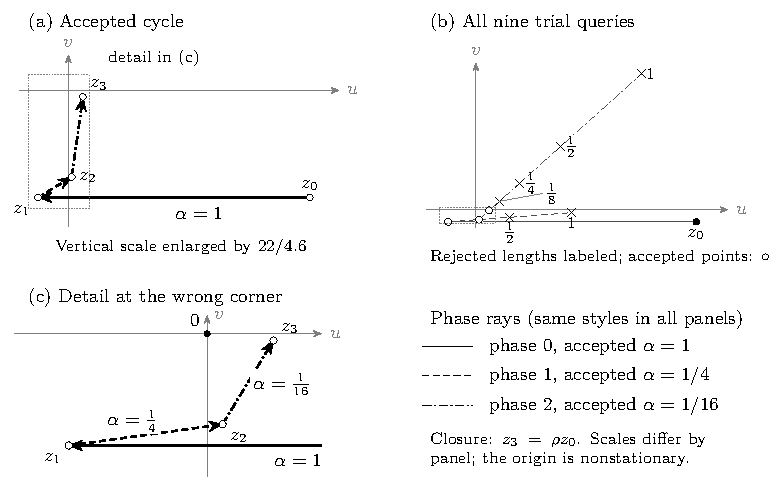
\includegraphics[width=\textwidth]{figures/cycle_trials.pdf}
\caption{The accepted three-step seed cycle (left), with closure
$z_3=\rho z_0$, and every rejected candidate point (right). The rendering
uses the rational center of the certified root box. It illustrates the
certified trial geometry; it is not a proof of exact equality or of
membership in the stable manifold used for the perturbed construction.}
\label{art:cycle-figure}
\end{figure}

Homogeneity and the two cycle closures now give an infinite induction:
\begin{equation}\label{art:cone_orbit}
 x_{3m+j}=\rho^mz_j,\qquad H_{3m+j}=\rho^mM_j,\qquad j=0,1,2.
\end{equation}
Each query in phase $j$ is $\rho^m$ times its base query. Gradients are
unchanged, function differences and gradient--step products scale by
$\rho^m$, and \eqref{art:failure_update} scales the updated matrix by
$\rho^m$. Thus every branch choice and every rejection is preserved, as
well as acceptance. The iterates converge to zero, but the direction
$w=(-1,16)^T$ satisfies
\[
 g_0^Tw=g_1^Tw=-1,\qquad g_2^Tw=-c+16d<-1.
\]
Hence $G(tw)=-t$ for $t\ge0$, so this limit is nonstationary.

\begin{corollary}[Coercive polyhedral global failure]\label{art:failure_polyhedral}
The same deterministic run, with $H_0=I$, fails for
\[
 \overline G(u,v)=\max\{u,-u-v/8,cu+dv,v-17\}.
\]
This function is coercive and has unique minimizer $(-1,16)$, with value
$-1$, while the run converges to the nonstationary origin with value zero.
\end{corollary}
\begin{proof}
At every query, \eqref{art:seed_query_bounds} and $0<\rho<1$ give
$v-17<0<G(u,v)$, so the fourth branch is inactive. The convex combination
of branches $0,1,3$ with weights $8/17,8/17,1/17$ is identically $-1$.
Equality in this lower bound forces all three branches to equal $-1$,
hence $(u,v)=(-1,16)$; the remaining branch is strictly smaller there.
If $\overline G(u,v)\le t$, then
$u\le t$, $v\le t+17$ and $-u-v/8\le t$, which also give lower bounds
on both coordinates. Every sublevel is therefore compact.
\end{proof}
This corollary concerns global failure at a wrong corner. The next step
places such corners arbitrarily near the true minimizer of one objective.

\subsection{Scalar interpolation with affine regions at every scale}
Let $\theta=1/16$, $a_n=\theta^n$, $\varepsilon=1/128$, and
$b_*=2c-32d\in(33,34)$. For $b\in\{2,b_*\}$ define
\[
 t_b=\frac{1-(1+\theta+\theta^2)/b}{1-\theta^2},\qquad
 v=\frac{\xi-t_b+\varepsilon}{2\varepsilon}.
\]
\[
 P_b(\xi)=
 \begin{cases}
 0&\xi\le t_b-\varepsilon,\\
 3v^2-2v^3&|\xi-t_b|<\varepsilon,\\
 1&\xi\ge t_b+\varepsilon,
 \end{cases}
 \quad J_b(\xi)=\int_0^\xi P_b(t)\,dt.
\]
The middle formula for $J_b$ is $2\varepsilon(v^3-v^4/2)$; its outer
formulas are zero and $\xi-t_b$. For
$b\theta a_n\le x\le ba_n$, set
\begin{equation}\label{art:upper_scalar}
 \varphi_b(x)=(\theta a_n)^3+
 ba_n^3(1-\theta)
 \{\theta^2\xi+(1-\theta^2)J_b(\xi)\},\qquad
 \xi=\frac{x/(ba_n)-\theta}{1-\theta}.
\end{equation}
Complete the definition by
\[
 \varphi_b(x)=
 \begin{cases}
 1-3(x+1)+3(x+1)^2&x<-1,\\
 -x^3&-1\le x\le0,\\
 1+x-b&x\ge b.
 \end{cases}
\]

\begin{lemma}[Scalar interpolation]\label{art:upper_scalar_lemma}
The functions $\varphi_b$ are convex, coercive and globally $C^{2,1}$,
are nonnegative, and vanish only at zero. They satisfy
\begin{align}
 0&\le\varphi_b''\le\max\{6,102/b\},\label{art:scalar_curvature}\\
 \varphi_b(ba_n+h)&=a_n^3+a_n^2h
       \qquad(|h|\le a_n/2).\label{art:scalar_plateau}
\end{align}
Their second derivatives are globally Lipschitz with constant
\[
 L_b=\max\{6,139264/(5b^2)\}.
\]
\end{lemma}
\begin{proof}
The ramp is monotone, $C^1$, and satisfies
$0\le P_b'\le96$ and $\int_0^1P_b=1-t_b$. On a positive interval,
\[
 \varphi_b'=a_n^2\{\theta^2+(1-\theta^2)P_b(\xi)\},\qquad
 \varphi_b''=\frac{a_n(1+\theta)}bP_b'(\xi).
\]
The identity
$\theta^2+(1-\theta^2)(1-t_b)=(1+\theta+\theta^2)/b$
gives matching values $\varphi_b(ba_n)=a_n^3$. The derivative is
constant near both ends of each interval, so the first two derivatives
also match, with values $a_n^2$ and zero at $ba_n$.

As $x\downarrow0$, the bounds $a_n\le x/(b\theta)$ on its interval
give $\varphi_b(x)=O(x^3)$, $\varphi_b'(x)=O(x^2)$ and
$\varphi_b''(x)=O(x)$. These match the negative cubic at zero.
The formulas also match through second order at $-1$ and $b$.
The derivative is negative on the negative half-line and positive on the
positive half-line; the outer formulas diverge to infinity. This proves
convexity, coercivity and the minimum assertions.

The constant-derivative lengths below and above $ba_n$, divided by $a_n$,
are
\[
 b(1-\theta)(1-t_b-\varepsilon),\qquad
 \frac{b(1-\theta)(t_b-\varepsilon)}\theta.
\]
Both exceed $1/2$ for $2\le b\le34$, by substitution in the displayed
rational formulas; the affine outer extension covers the upper side when
$n=0$. This proves \eqref{art:scalar_plateau}.
Finally $|P_b''|\le3/(2\varepsilon^2)$ in each ramp, so differentiation
once more gives $|\varphi_b'''|\le139264/(5b^2)$ there. The negative
cubic has third derivative of magnitude six. Continuity of
$\varphi_b''$ permits summing the Lipschitz estimates over finitely many
joins away from zero; taking limits at zero covers the infinitely many
accumulating joins and gives the global bound.
\end{proof}

\subsection{One objective and a uniform induction over all queries}
Define
\begin{equation}\label{art:upper_objective}
 F(u,v)=\max\{\varphi_2(u),\varphi_2(-u-v/8),
                    \varphi_{b_*}(cu+dv),v\}.
\end{equation}
The Hessian of each of the first three branches is a nonnegative scalar
multiple of $g_ig_i^T$. Equation~\eqref{art:scalar_curvature} gives the
upper bounds $51$, $51(65/64)<52$, and $12$, respectively, on their
operator norms; the last branch has zero Hessian. Their Hessians are
globally Lipschitz because $\varphi_b''$ is Lipschitz and the arguments
are linear. The first two scalar arguments are independent, so their
coercivity makes every sublevel of $F$ compact. Nonnegativity and their
unique scalar zeros show $F(x)=0$ exactly at $x=0$. At zero the first
three gradients vanish and the last is $(0,1)^T$, giving
$F'(0;h)=\max\{0,h_2\}$; thus the minimizer is nonsmooth.

Let $p_n=a_n(2,-32)^T$. The first two scalar arguments at $p_n$ equal
$2a_n$, and the third equals $b_*a_n$. Consequently
\begin{equation}\label{art:upper_local_model}
 F(p_n+h)=a_n^3+a_n^2G(h)
 \quad\hbox{if } |g_i^Th|\le a_n/2 (i=0,1,2).
\end{equation}
Indeed, the first three branches are on their affine regions and each
has value at least $a_n^3/2$. The first two slab inequalities imply
$|h_1|\le a_n/2$ and $|h_2|\le8a_n$, so the fourth branch is negative.
In particular $F(p_n)=a_n^3$ and
$F'(p_n;(-1,16)^T)=-a_n^2<0$.

\begin{proof}[Proof of Theorem~\ref{art:local-failure}]
For $n\ge1$ take $x_0^{(n)}=p_n+a_n^2z_0$ and $H_0=I$. We claim that
\begin{equation}\label{art:upper_orbit}
 x_{3m+j}^{(n)}=p_n+a_n^2\rho^mz_j,\qquad
 H_{3m+j}^{(n)}=\rho^mM_j,\qquad j=0,1,2.
\end{equation}
At a current point of this form its gradient is $a_n^2g_j$. Every trial
on the finite candidate list therefore has the form
$p_n+a_n^2\rho^mz_{\rm trial}$. Equation~\eqref{art:seed_query_bounds}
gives
\[
 |g_i^T(a_n^2\rho^mz_{\rm trial})|<3a_n^2
 \le3a_n/16<a_n/2.
\]
Thus \eqref{art:upper_local_model} is valid at every candidate query,
not only the final accepted one. Unique activity is preserved, and
\[
 F(p_n+a_n^2\rho^mz_{\rm trial})
   =a_n^3+a_n^4\rho^mG(z_{\rm trial}),\qquad
 \nabla F=a_n^2g_{\rm active}.
\]
The additive constant cancels in Armijo. Function differences and
gradient--step products are the seed quantities multiplied by the same
positive factor $a_n^4\rho^m$. The actual search therefore traverses
exactly the candidate list and makes the same strict decisions.
In \eqref{art:failure_update}, the projection factors are unchanged and
the rank-one term has factor $\rho^m$. The cycle closures prove the next
point and matrix identities, completing the induction.

The finite matrices are positive definite. Equation~\eqref{art:upper_orbit}
gives convergence to $p_n$ and strict descent to $a_n^3>0$.
Since the base query set is finite, the norm of every query is bounded by
\[
 a_n\|(2,-32)\|+a_n^2\max_{\text{base points and queries}}\|z\|,
\]
which tends to zero. The starting points also tend to zero. All other
claims were proved directly from \eqref{art:upper_objective}.
\end{proof}

\section{Synthesis, verification and the remaining questions}\label{art:verification}

The mixed quadratic--absolute-value benchmark now has a whole-sequence
answer: every admissible full-BFGS run for $u^2+|v|$ converges to its unique
minimizer. The same centered-family argument gives global convergence for
smooth-plus-sublinear objectives whose compact initial sublevels lie in the
region of the structural representation,
and recovers the known Euclidean-norm result inside the broader coercive
homogeneous class. Locally, finite polyhedral geometry controls the inward
model error. The planar theorem goes further: a moving comparison field
handles curved switches in the three-quadratic example even though its radial
secant condition fails. These are objective-based convergence results, with
their distinct compactness and geometric assumptions intact.

The counterexamples place a different limit on deterministic guarantees.
They exclude a neighborhood in which every admissible start
succeeds for the specified unit-first search, both for finite maxima of
convex $C^{2,1}$ branches with bounded Hessians and, independently, for the
stated uniformly strongly convex $C^{1,1}$ regime. Simpler polyhedral and
quadratic-plus-maximum examples establish global failure near a wrong corner;
the local embeddings are needed to place bad starts arbitrarily near the
objective's own minimizer. The proof follows the actual full update and every
line-search query, so the failure is an algorithmic trajectory, not only a
prescribed sequence of accepted points.

The common analytical advance is a route around a full spectral description
of the BFGS matrices. The principal-minor hierarchy constrains the decrease
metric even while the matrices degenerate. A comparison energy then converts
those constraints into progress whenever its directions continue to see the
remaining objective gap with controlled secant and transport costs. The radial,
finite-partition and planar arguments provide different ways of meeting these
requirements. Their success does not make the requirements necessary, or turn
an affine-critical obstruction into a universal dynamical classification.

These distinctions leave precise questions. The two local negatives do not
give a counterexample with finitely many uniformly strongly convex $C^2$
branches through the minimizer; the planar positive theorem settles a
nondegenerate subclass, not that entire class. Nor do exceptional deterministic
starts establish failure with positive probability. The accumulating local
constructions do not have a finite semialgebraic description. The almost-sure
stationarity, all-trial-value rate and spectral-identification assertions in
Lewis--Overton's challenge~\cite[Challenge~7.1]{LO} therefore remain outside
the conclusions proved here. We also distinguish convergence of an infinite
admissible run from a guarantee of indefinite differentiable execution; a
zero gradient is successful termination in this paper.

\paragraph{Formal verification and reproducibility.}
The companion records Lean~4.19.0 proofs with pinned mathlib, exact
statement-to-source correspondence, and compiler and transitive-axiom audit
logs. The permitted foundational dependencies are propositional
extensionality (\texttt{propext}), classical choice
(\texttt{Classical.choice}) and quotient soundness (\texttt{Quot.sound}).
The audits reject \texttt{sorryAx}, custom mathematical axioms and reachable
unsafe or partial proof artifacts. The principal-minor theorem concerns the
actual matrices and determinants, and the negative proofs include the search
decisions and all-query induction. The rational certificate and the article's
proofs can also be read independently of Lean. Formal checking supports these
precise claims; it does not establish foundational consistency, publication
priority, fidelity of every prose paraphrase, or floating-point robustness.
The kernel and execution environment remain trusted, and author-side
correspondence reviews are separate from independent human peer review.

\paragraph{AI assistance and author review.}
The accompanying source tree contains the article, complete companion,
figure-generation code, exact certificates and Lean project. Large language
models assisted theorem development, proof reconstruction, formalization,
literature searches, software and writing. This assistance was substantive;
it was not limited to grammar editing. Human authors must review the claims,
citations, novelty assessment and disclosure before submission. This
author-review edition asserts no author consent, independent human review,
affiliations, grants or public archival identifier.

\appendix
\normalsize
\section{The BFGS compression calculation}\label{art:matrix-algebra}

\begin{lemma}\label{art:gram-compression}
Under the assumptions of Theorem~\ref{art:minor-hierarchy}, let $Z$ have
$j$ orthonormal columns, $1\le j\le n$. Then
\[
 \det(Z^TH_+Z)\le
 \frac{\det\operatorname{Gram}_H(y,Z)}{\beta^2q}
       +\frac\alpha\beta\det(Z^THZ).
\]
For $j=n$, $\det H_+=(\alpha/\beta)\det H$.
\end{lemma}
\begin{proof}
Put $v=Hg$, $\kappa=g^THy=-\beta q$ and
$P=I-vy^T/\kappa$. Since $y^Ts=\alpha\beta q$, the update becomes
\[
 H_+=\mathcal F+\frac{\alpha}{\beta q}vv^T,
 \qquad \mathcal F=PHP^T.
\]
Write
\[
 \begin{gathered}
 A=Z^THZ\succ0,\quad a=Z^THg,\quad b=Z^THy,\quad r=y^THy,\\
 u=a^TA^{-1}a,\quad w=a^TA^{-1}b,\quad z=b^TA^{-1}b.
 \end{gathered}
\]
Then
\[
 Z^T\mathcal FZ
 =A-[a\ b]
 \begin{pmatrix}-r/\kappa^2&1/\kappa\\1/\kappa&0\end{pmatrix}
 [a\ b]^T.
\]
The identity $\det(I+UV)=\det(I+VU)$ reduces its determinant to a
$2\times2$ determinant. Expanding gives
\begin{equation}\label{art:compression-determinant}
 \det(Z^T\mathcal FZ)
 =\frac{\det A}{\kappa^2}
       \bigl((\kappa-w)^2+u(r-z)\bigr).
\end{equation}
Schur complements give, independently,
\begin{align*}
 \det\operatorname{Gram}_H(y,Z)&=\det A(r-z),\\
 \det\operatorname{Gram}_H(g,y,Z)
 &=\det A\bigl((q-u)(r-z)-(\kappa-w)^2\bigr).
\end{align*}
Both are Gram determinants and hence nonnegative, including when their
column families are dependent. Combining these identities yields
\[
 \det(Z^T\mathcal FZ)
 =\frac{q\det\operatorname{Gram}_H(y,Z)
             -\det\operatorname{Gram}_H(g,y,Z)}{\beta^2q^2}
 \le\frac{\det\operatorname{Gram}_H(y,Z)}{\beta^2q}.
\]

Adding $\rho aa^T$ to the compression changes the coefficient $r/\kappa^2$
by $\rho$. The same $2\times2$ expansion therefore changes its determinant
by exactly $\rho\det A\,u$. No invertibility of
$Z^T\mathcal FZ$ is used. For $\rho=\alpha/(\beta q)$, the Schur
complement of $A$ in $\operatorname{Gram}_H(g,Z)$ gives $0\le u\le q$,
so the increase is at most $(\alpha/\beta)\det A$.
This proves the inequality.

When $j=n$, $Z$ is an orthogonal basis and $u=q$, $w=\kappa$, $z=r$.
Equation~\eqref{art:compression-determinant} then vanishes, while the
rank-one increase is exactly $(\alpha/\beta)\det A$.
Orthogonal invariance gives the stated determinant identity.
\end{proof}

\section{The algebraic seed and its finite rational certificate}
\label{art:seed_certificate}

This appendix gives the objects and finite inequalities needed for
Lemma~\ref{art:seed_cycle}. All decimals defining a box are terminating
rationals. No rounded point is substituted for a root or an infinite orbit.

\subsection{Existence and uniqueness of the defining root}
Put
\begin{align*}
 U&=127c+16d,&V&=16c-127d-16,&R&=c-8d,\\
 K&=8c^2+8d^2+d-8,&T&=c^2-c+d^2,&Y&=(c-1)^2+d^2,
\end{align*}
and let
\begin{equation}\label{art:seed_polynomials}
 P(c,d)=
 \begin{pmatrix}264192RK-UV(U+129)\\16VTK-RUY\end{pmatrix}.
\end{equation}
The root is specified by $P(c,d)=0$ and
$\|(c,d)-\bar r\|_\infty\le10^{-30}$, where
\begin{align*}
 \bar r_1&=0.31848142762711863064645131250290703717912205023605,\\
 \bar r_2&=-1.02523211967574872548135087001300414284511909318444.
\end{align*}

\begin{lemma}[Rational root certificate]\label{art:root_certificate}
This closed box contains exactly one root. On the box all of
$U,V,R,K,T,Y,U+129$ are positive, and \eqref{art:seed_rho} holds.
\end{lemma}
\begin{proof}
Let $D=DP(\bar r)$ and define its inverse by the ordinary two-by-two
adjugate formula $A=\operatorname{adj}(D)/\det D$.
The following finite rational certificate uses only the coefficients of
\eqref{art:seed_polynomials} and the two displayed rationals:
\begin{equation}\label{art:root_arithmetic}
 \det D\ne0,\qquad
 \max_i |(AP(\bar r))_i|<10^{-50},\qquad
 \max_i\sum_{2\le|\nu|\le5}|a_{i,\nu}|\,|\nu|\le7000,
\end{equation}
where, for $\nu=(\nu_1,\nu_2)$,
\[
 a_{i,\nu}=-\frac{1}{\nu_1!\nu_2!}
     \sum_{j=1}^2 A_{ij}\,\partial^\nu P_j(\bar r).
\]
These formulas specify every rational in the certificate: the index set
contains the eighteen monomials of degrees two through five. The bounds
in \eqref{art:root_arithmetic} follow by substituting the rational center,
differentiating the displayed polynomials, and clearing positive
denominators in the three comparisons. Thus they are finite integer
inequalities, rather than tolerances for a numerically computed root.

For completeness, their analytic consequence follows directly.
The centered residual map $N(h)=h-AP(\bar r+h)$ has the exact expansion
\[
 N_i(h)=-(AP(\bar r))_i+
           \sum_{2\le|\nu|\le5}a_{i,\nu}h^\nu;
\]
its linear part vanishes because $AD=I$.
On $\|h\|_\infty,\|k\|_\infty\le r=10^{-30}$, telescoping the
factors of each monomial gives
$|h^\nu-k^\nu|\le|\nu|r\|h-k\|_\infty$, since $r\le1$ and
$|\nu|\ge2$. Hence $N$ has Lipschitz constant at most $7000r$ and
\[
 \|N(h)\|_\infty\le10^{-50}+7000r^2<r.
\]
The closed box is complete, so contraction gives a unique fixed point.
Since $A$ is invertible, this is exactly a root of $P$.
This is the standard preconditioned-residual principle; compare
Rump~\cite[Theorem~13.3]{NEG_RUMP10}.

The root box lies in
$318/1000<c<319/1000$ and $-1026/1000<d<-1025/1000$.
Substitution gives positivity of the stated factors. For example,
\[
 \frac{2397}{100}\le U\le\frac{24113}{1000},\quad
 \frac{119263}{1000}\le V\le\frac{59703}{500},\quad
 \frac{4259}{500}\le R\le\frac{8527}{1000}.
\]
Multiplying positive endpoints in $129R/[V(U+129)]$ gives
$60/1000<\rho<61/1000$. In particular all divisions used below are valid.
\end{proof}

\subsection{The matrix identity}
\begin{proof}[Proof of the algebraic part of Lemma~\ref{art:seed_cycle}]
The first update in \eqref{art:seed_matrices} is immediate from
$s_0=(-1,0)^T$ and $g_1-g_0=(-2,-1/8)^T$.
For arbitrary $(c,d)$ with the positive factors above, put
\[
 \beta=\frac{66048RK}{UV(U+129)},\quad
 \gamma=\frac{VTK}{RUY},\quad
 \widetilde\rho=\frac{2064TK}{U(U+129)Y}.
\]
The rational identities obtained from \eqref{art:failure_update} are
\begin{equation}\label{art:closure_identity}
 \mathcal B(\mathcal B(M_1,g_1,g_2,\beta),g_2,g_0,\gamma)
     =\widetilde\rho I,\qquad
 -\gamma\mathcal B(M_1,g_1,g_2,\beta)g_2
     =\widetilde\rho(g_0-g_2).
\end{equation}
Here is a way to check the identities without guessing matrix entries.
The middle update is $C+\beta E$, because its two projection factors
are independent of the step length and its rank-one term is linear in
that length. Requiring $(C+\beta E)g_2$ to be parallel to $g_0-g_2$
gives a linear equation for $\beta$; substitution of $M_1,g_1,g_2$
gives the displayed value. For a unit vector $w\perp(g_0-g_2)$,
substitution gives $w^T(C+\beta E)w=\widetilde\rho$.
With the displayed $\gamma$, the last step is
$\widetilde\rho(g_0-g_2)$. Its projection factors are the orthogonal
projector onto $(g_0-g_2)^\perp$, and its rank-one term is
$\widetilde\rho$ times the complementary projector. Their sum is
$\widetilde\rho I$, proving \eqref{art:closure_identity}.
Each substitution is a rational identity and can equivalently be
checked by clearing their nonzero denominators and expanding.

Equations~\eqref{art:seed_polynomials} give exactly
$\beta=1/4$ and $\gamma=1/16$. Moreover,
\[
 \widetilde\rho-\rho=
 \frac{2064R}{V(U+129)}\left(\gamma-\frac1{16}\right)=0.
\]
This gives the matrix and displacement closures. The formula for $z_0$
gives $s_0+s_1+s_2=-(1-\rho)z_0$.
The strict inequalities below imply
$(g_{j+1}-g_j)^Ts_j>0$ at each phase. Positive definiteness follows
inductively from the full update: its two nonnegative quadratic terms
cannot both vanish on a nonzero vector when $y^Ts>0$.
\end{proof}

\subsection{Sound enclosure of every query}
An interval $[a,b]$ encloses the corresponding real quantity. Addition,
negation, multiplication and reciprocal are evaluated by
\begin{align*}
 [a,b]+[c,d]&=[a+c,b+d],\qquad -[a,b]=[-b,-a],\\
 [a,b][c,d]&=[\min(ac,ad,bc,bd),\max(ac,ad,bc,bd)],
\end{align*}
and $[a,b]^{-1}=[1/b,1/a]$ when $0\notin[a,b]$.
These inclusion rules follow from order on the reals; induction on a
rational expression proves the soundness of every resulting bound.
All endpoints used here are rational, so no directed floating-point
rounding is needed.

For the query calculation it suffices to use the larger box
\begin{equation}\label{art:query_box}
 c\in\frac{[318481,318482]}{10^6},\quad
 d\in\frac{[-1025233,-1025232]}{10^6},\quad
 \rho\in\frac{[6019,6021]}{10^5}.
\end{equation}
The first two inclusions follow from the root box; substitution in
\eqref{art:seed_rho}, with positive denominator, gives the third.
Evaluate $z_j$ from \eqref{art:seed_points} and use
\[
 p_0=(-1,0)^T,\quad p_1=(127/256,1/16)^T,\quad
 p_2=16\rho(1-c,-d)^T.
\]
For a row with active index $i$, set $q=z_j+\alpha p_j$ and evaluate
the following rational expressions by the inclusion rules:
\[
 (g_i-g_k)^Tq (k\ne i),\quad -\alpha g_j^Tp_j,\quad
 \begin{cases}
 g_j^Tz_j+\alpha g_j^Tp_j/3-g_i^Tq,&\text{acceptance},\\
 g_i^Tq-g_j^Tz_j,&\text{rejection}.
 \end{cases}
\]
For an acceptance also evaluate $\alpha g_i^Tp_j$.
Every expression in its row is strictly greater than the following
positive rational lower bound, in the order of Table~\ref{art:trial_table}:
\begin{equation}\label{art:query_lower_bounds}
 \frac1{10^4}(729, 2417, 145, 75, 5964, 2682, 1041, 221, 20).
\end{equation}
The same interval operations give the value enclosures in that table.
For the three base points, the designated active gaps are positive as
well. Evaluating $3\pm g_i^Tq$ for every $i$, $2-q_2$, and the
designated active value $g_i^Tq$ gives positive lower bounds for all base
points and all nine queries. This proves
\eqref{art:seed_query_bounds}. All inputs, expressions, interval rules
and output bounds of this finite certificate are now specified. The
strict active gaps also give differentiability on a neighborhood of
each query. Together with the matrix identities, these calculations
complete the proof of Lemma~\ref{art:seed_cycle}.

\section{Positive lower curvature through a perturbed cycle}
\label{art:lower_curvature}

Theorem~\ref{art:local-failure-lower} uses a different regularity balance
from Theorem~\ref{art:local-failure}. Adding a positive quadratic changes
the seed orbit, so exact homogeneity alone no longer supplies a trajectory.
We first prove persistence on a stable manifold and then copy one entire
perturbed orbit at all scales. The first step yields a global failure
from a suitable matrix; the copying step makes bad starts approach the
minimizer of one fixed objective; a final fixed change of coordinates
makes their common initial matrix the identity. The price of retaining
a positive lower curvature bound is the loss of second differentiability
of the branches at the accumulation point. Throughout this appendix the
line-search constants are $c_1=10^{-4}$ and $c_2=1/2$.

\subsection{A strongly convex global example}
A common positive quadratic leaves the active-branch geometry unchanged
and makes every sublevel compact. It perturbs the gradients, however, so
the homogeneous seed is no longer an exact orbit. Close to the corner,
the quadratic gradient is small relative to the fixed slopes. The task
is to turn this smallness into an exact infinite trajectory, with every
rejection and acceptance retained.

Use the fixed slopes of Appendix~\ref{art:seed_certificate} and let
\[
 Q_\mu(x)=\tfrac\mu2\|x\|^2+G(x),\qquad\mu>0.
\]
The vector
\[
 \bar g=\frac{(1,-16)^T}{257}
        =\frac{129}{257}g_0+\frac{128}{257}g_1
\]
is the least-norm point of $\operatorname{conv}\{g_0,g_1,g_2\}$:
$g_0^T\bar g=g_1^T\bar g=\|\bar g\|^2=1/257$, whereas
$g_2^T\bar g>1/257$. Therefore the unique minimizer is
\begin{equation}\label{art:quadratic_minimizer}
 x_*=-\bar g/\mu,\qquad \min Q_\mu=-1/(514\mu).
\end{equation}
At $x_*$ the first two branches tie with distinct gradients, so the
minimizer is nonsmooth. At zero the subdifferential is the nonstationary
triangle of the original seed.

\begin{proposition}[A perturbed bad orbit]\label{art:quadratic_failure}
For every $\mu>0$ and every neighborhood $V$ of zero, some initial state
$(x_0,H_0)$, $H_0\succ0$, produces a deterministic full-BFGS run on
$Q_\mu$ converging to zero, with positive objective values decreasing to
zero. Its accepted lengths repeat $1,1/4,1/16$, and all accepted and
rejected query points are differentiable and belong to $V$.
\end{proposition}

The right object for persistence is the three-step return map after
dividing out the shrinking scale. The homogeneous cycle becomes a fixed
point on the boundary where that scale is zero. We will verify that it
is hyperbolic and that its stable manifold enters the positive-scale
region. This gives exact perturbed orbits; closeness of a finite
floating-point trajectory would not. To prove the proposition, use
normalized coordinates
\[
 x=\tau z,\qquad H=\tau M(b,e),\qquad
 M(b,e)=\begin{pmatrix}1&b\\b&e\end{pmatrix},\qquad\tau>0.
\]
The boundary seed is $P_*=(z_0,0,1,0)$ in coordinates $(z,b,e,\tau)$.
Keep the input $\tau$ fixed during three substeps. Starting with
$(Z,M)=(z,M(b,e))$, for $j=0,1,2$ perform
\begin{align}
 \gamma_j&=g_j+\mu\tau Z,\qquad S=-\alpha_jM\gamma_j,
       \qquad Z^+=Z+S,\label{art:lower_return_substep}\\
 Y&=g_{j+1}-g_j+\mu\tau S,\notag\\
 M^+&=\left(I-\frac{SY^T}{Y^TS}\right)M
          \left(I-\frac{YS^T}{Y^TS}\right)+\frac{SS^T}{Y^TS}.\notag
\end{align}
with cyclic gradient indices and $\alpha=(1,1/4,1/16)$.
For the resulting $(Z_3,M_3)$, let $r=(M_3)_{11}$ and define
\begin{equation}\label{art:lower_return}
 \mathcal T_\mu(z,b,e,\tau)
 =\left(Z_3/r, (M_3)_{12}/r, (M_3)_{22}/r, \tau r\right).
\end{equation}
The seed closure gives $\mathcal T_\mu(P_*)=P_*$ and $r(P_*)=\rho$.
All denominators are nonzero there. Hence the map is real analytic on an
open neighborhood of $P_*$, using negative $\tau$ only to define this
analytic extension.

\begin{lemma}[Implementation and hyperbolicity]\label{art:lower_hyperbolic}
On a sufficiently small neighborhood of $P_*$, positive-$\tau$ states
follow exactly the three query lists of Table~\ref{art:trial_table} under
the actual algorithm, and \eqref{art:lower_return} is their return map.
Its derivative has eigenvalues
\[
 \rho^{-1},\quad\rho^{-1},\quad\lambda_s,\quad\lambda_u,\quad\rho,
 \qquad .038<\lambda_s<.039,\quad1.564<\lambda_u<1.565.
\]
The stable eigenspace contains a vector whose $\tau$ coordinate is one.
\end{lemma}
\begin{proof}
At a query $\tau Z$, the value divided by $\tau$ is
$G(Z)+\mu\tau\|Z\|^2/2$ and the gradient is $g_i+\mu\tau Z$.
The common quadratic does not affect which slope is active. All finite
branch gaps and normalized search comparisons are continuous in the
normalized state. The strict seed margins therefore persist on a common
neighborhood. The physical step and secant are exactly the ones in
\eqref{art:lower_return_substep} after restoring the scale, proving
agreement with the actual update and the entire search tree.

At $\tau=0$ the matrix return is independent of $z$. Let $J$ be the
derivative at $(b,e)=(0,1)$ of its normalized shape map.
The following rational enclosures specify the spectral certificate:
\begin{equation}\label{art:shape_certificate}
 10^{10}J\ \in
 \begin{pmatrix}
 [11123986249,11123986253]&[6459701025,6459701029]\\
 [7515015701,7515015708]&[4905136882,4905136890]
 \end{pmatrix}.
\end{equation}
They are obtained by differentiating the rational substeps
\eqref{art:lower_return_substep} at $\tau=0$, then applying the interval
rules of Appendix~\ref{art:seed_certificate} to
\begin{align*}
 c&\in[318481427627118,318481427627119]/10^{15},\\
 d&\in[-1025232119675749,-1025232119675748]/10^{15}.
\end{align*}
Both intervals contain the defining root box. This is a finite rational
derivative calculation: for a product use
$D(ab)=a\,Db+b\,Da$, and for an inverse use
$D(a^{-1})=-a^{-2}Da$, with denominators bounded away from zero.
Substitution of \eqref{art:shape_certificate} in
$p(\lambda)=\lambda^2-\operatorname{tr}(J)\lambda+\det J$ gives
\[
 p(.038)>0,\qquad p(.039)<0,\qquad
 p(1.564)<0,\qquad p(1.565)>0.
\]
These rational sign comparisons locate two distinct real roots and exhaust
the degree-two polynomial; no numerical eigenvector is used.

At $\tau=0$, $Z_3=z+v(b,e)$ and $r$ is independent of $z$.
The last coordinate of the return is $\tau r$. Thus its full derivative
has the block form
\[
 D\mathcal T_\mu(P_*)=
 \begin{pmatrix}
 \rho^{-1}I_2&C&\mu a\\0&J&\mu b'\\0&0&\rho
 \end{pmatrix}.
\]
The unspecified blocks are finite derivatives of the displayed rational
map and do not affect its spectrum. None of the five eigenvalues is zero
or has modulus one. Moreover $\rho$ is not an eigenvalue of the upper
left four-dimensional block. Assigning last coordinate one and solving
the remaining four linear equations gives a $\rho$-eigenvector. This
proves the last assertion and the lemma.
\end{proof}

\begin{proof}[Proof of Proposition~\ref{art:quadratic_failure}]
The inverse function theorem makes the return map a local diffeomorphism.
The classical local stable-manifold theorem provides a two-dimensional
smooth stable manifold through $P_*$, tangent to the stable eigenspace;
\preprintcite{DY} gives an exposition of this principle and its graph
transform proof. By the last assertion of
Lemma~\ref{art:lower_hyperbolic}, this manifold contains points with
arbitrarily small positive $\tau$.
Choose such a point whose forward return orbit stays in the implementation
neighborhood and tends to $P_*$. Shrinking the neighborhood keeps $r>0$
and $M(b,e)\succ0$, so $\tau^+=\tau r$ preserves positivity. The actual
intermediate matrices remain positive definite by positive curvature.

The physical iterates are $x_{3m}=\tau_mz_m\to0$. Intermediate points
and all queries are $\tau_m$ times bounded continuous functions of the
normalized state, so they tend to zero too. Their normalized objective
values stay positive by the seed's strict positivity. Armijo makes the
values decrease to zero, which exceeds \eqref{art:quadratic_minimizer}.
The initial stable-manifold point can be taken sufficiently close to
$P_*$ that the entire local stable orbit, and hence every physical query,
lies in the prescribed $V$. This proves the proposition. The initial
matrix is supplied by the stable-manifold point, not presumed to be
identity or obtained by rounded forward shooting.
\end{proof}

\subsection{An accumulation embedding with four strongly convex branches}
The previous proposition places a bad orbit near its wrong corner,
whereas the desired local counterexample needs bad starts near the
minimizer. We therefore place shrinking copies around centers $p_n$
converging to that minimizer. The spatial factor will be $a_n$, and the
objective factor $a_n^2$, which preserves the same inverse matrix by
\eqref{art:matched-scaling}. To accommodate the common quadratic, the
three scalar branch slopes are shifted so that the quadratic cross term
restores the original seed gradients inside every copy.

The scalar interpolation must have value $a_n^2$ and derivative $a_n$
at its $n$th node, with an affine neighborhood wide enough to contain
all seed queries after scaling. A monotone cubic ramp between these
plateaux gives a convex function with Lipschitz derivative. The node
slopes divided by the node positions stay of order one, so this
construction need not, and will not, have a second derivative at zero.

Fix
\begin{gather*}
 \mu=1/4096,\qquad c_*=(2,-32)^T,\qquad q_i=g_i-\mu c_*,\\
 b_i=q_i^Tc_*,\qquad r=1/128,\qquad a_n=r^n.
\end{gather*}
Here $b_0=b_1=1791/1024$ and $1.7<b_i<34$. For each of the two distinct
values of $b_i$, set
\[
 t_b=\frac{1-(1+r)/b}{1-r},\qquad\varepsilon=1/1024.
\]
Use the same cubic ramp $P_b$ and primitive $J_b$ as in
\eqref{art:upper_scalar}, with this center and width. For
$ba_{n+1}\le x\le ba_n$ put
\begin{equation}\label{art:lower_scalar}
 \psi_b(x)=(ra_n)^2+ba_n^2(1-r)
       \{r\xi+(1-r)J_b(\xi)\},\qquad
 \xi=\frac{x/(ba_n)-r}{1-r}.
\end{equation}
Set $\psi_b(0)=0$, $\psi_b(x)=x^2/2$ for $x<0$, and
$\psi_b(x)=1+x-b$ for $x\ge b$.

On each positive interval,
\[
 \psi_b'=a_n\{r+(1-r)P_b(\xi)\},\qquad
 \psi_b''=P_b'(\xi)/b,\qquad0\le P_b'\le768.
\]
The identity $r+(1-r)(1-t_b)=(1+r)/b$ matches node values and
derivatives. Their values are $a_n^2$ and $a_n$, respectively.
The positive derivative is monotone and constant near every node.
Its derivative slopes are uniformly bounded, so summing over intervals
and taking a limit at zero proves that $\psi_b$ is globally $C^{1,1}$,
convex and coercive, nonnegative with unique zero at the origin.
The two constant-derivative lengths, divided by $a_n$, are
\[
 b(1-r)(1-t_b-\varepsilon),\qquad
 b(1-r)(t_b-\varepsilon)/r,
\]
both greater than $1/2$ for these values of $b$. Consequently
\begin{equation}\label{art:lower_plateau}
 \psi_b(ba_n+h)=a_n^2+a_nh\qquad(|h|\le a_n/2).
\end{equation}
At zero, the difference quotients of $\psi_b'$ along $ba_n$ and
$(b+1/4)a_n$ equal $1/b$ and $1/(b+1/4)$, respectively. Thus its second
derivative at zero does not exist.

Define
\begin{equation}\label{art:lower_objective}
 \begin{aligned}
 f_i(x)&=\tfrac\mu2\|x\|^2+\psi_{b_i}(q_i^Tx)\qquad(i=0,1,2),\\
 f_3(x)&=\tfrac\mu2\|x\|^2+x_2,\qquad F=\max_i f_i.
 \end{aligned}
\end{equation}
Each branch is globally $\mu$-strongly convex and $C^{1,1}$.
For the first three branches, the gradient-Lipschitz constants are at most
$L_i=\mu+\max\{1,768/b_i\}\|q_i\|^2$. Direct substitution of the
rational root bounds gives $L_0<439$, $L_1<446$ and $L_2<27$; hence
$512$ is a common constant, also covering the fourth branch.
Since $F(x)\ge\mu\|x\|^2/2$ with equality zero at the origin, the
sublevels are compact and the minimizer is unique. The first three
gradients at zero vanish, whereas the fourth is $(0,1)^T$, so the
minimizer is nonsmooth.

At a differentiable point of a finite maximum of $L$-smooth functions,
all active gradients agree. Inactive branches stay inactive locally;
taking the maximum of the active upper Taylor bounds therefore gives
the local upper Taylor bound with constant $L$. Applying this with
$L=512$ and combining it with strong convexity proves
\[
 \mu I\preceq\nabla^2F(x)\preceq512I
 \quad\text{whenever }F\text{ is twice differentiable}.
\]
This does not require a globally Lipschitz gradient for the maximum itself.

\subsection{Copying one entire orbit and fixing the initial matrix}
Let $p_n=a_nc_*$ and $C_*=1+\mu\|c_*\|^2/2$.
For $y$ in a fixed sufficiently small neighborhood of zero,
\eqref{art:lower_plateau} yields
\begin{equation}\label{art:lower_local_model}
 F(p_n+a_ny)=a_n^2\{C_*+Q_\mu(y)\}\qquad(n\ge1).
\end{equation}
Indeed, $|q_i^Ty|\le1/2$ puts each old branch in its affine scalar
region, and expansion of the common quadratic uses $q_i+\mu c_*=g_i$.
The fourth branch is inactive there: its residual $a_n(-32+y_2)$ is
negative, while each old scalar residual is at least $a_n^2/2$.

Choose, by Proposition~\ref{art:quadratic_failure}, one bad orbit
$(\bar x_k,\bar H_k)$ all of whose queries lie in this neighborhood.
For every $n$, start at $p_n+a_n\bar x_0$ with the same matrix
$\bar H_0$. Induction on the actual query tree gives
\[
 x_k^{(n)}=p_n+a_n\bar x_k,\qquad H_k^{(n)}=\bar H_k.
\]
This is \eqref{art:matched-local-model} with spatial factor $a_n$
and objective factor $a_n^2$. The covariance calculation
\eqref{art:matched-scaling} preserves the matrix, while function
differences and directional products acquire the same positive factor.
Thus each rejection, acceptance and updated matrix is preserved. Equation~\eqref{art:lower_local_model} applies to every
query because the whole chosen seed orbit lies in its domain.
Thus $x_k^{(n)}\to p_n$ and
$F(x_k^{(n)})\downarrow a_n^2C_*>0$. The three active gradients at
$p_n$ are $a_ng_i$, whose convex hull excludes zero.
All query norms are at most
$a_n(\|c_*\|+\sup_{\rm seed\ queries}\|\bar x\|)\to0$.

The seed supplied by the stable manifold has a positive-definite initial
matrix $\bar H_0$, common to every copy. Identity initialization is
obtained by changing coordinates once for the whole objective and the
whole sequence of starts, rather than selecting a different objective
for each start. Set $A=\bar H_0^{1/2}$ and $\widetilde F(z)=F(Az)$.
The coordinate identities
\[
 \widetilde g=A^Tg,\qquad \widetilde H=A^{-1}HA^{-T},\qquad
 \widetilde s=A^{-1}s
\]
preserve both scalar line-search tests and
\eqref{art:failure_update}; see also~\cite[Section~2]{LO}.
They give $\widetilde H_0=I$ for this one fixed transformation.
Strong-convexity and smoothness constants become
$\underline\mu=\mu\lambda_{\min}(\bar H_0)$ and
$\overline L=512\lambda_{\max}(\bar H_0)$.
All locality and differentiability statements persist under the
invertible linear map. This proves
Theorem~\ref{art:local-failure-lower}.

% Published works cited in the actual article assembly.
\begin{thebibliography}{99}

\bibitem{LO} A. S. Lewis and M. L. Overton. \emph{Nonsmooth optimization via quasi-Newton methods}. Mathematical Programming 141 (2013), 135--163; published online 16 February 2012. \url{https://doi.org/10.1007/s10107-012-0514-2}.

\bibitem{WW} D. Wachsmuth and G. Wachsmuth. \emph{A simple proof of the Baillon--Haddad theorem on open subsets of Hilbert spaces}. Journal of Convex Analysis 30(4) (2023), 1319--1328. \url{https://journalofconvexanalysis.com/articles/jca30059/}.

\bibitem{BG} B. Gebken. \emph{Technical Results on the Convergence of Quasi-Newton Methods for Nonsmooth Optimization}. Journal of Optimization Theory and Applications 209, article 57 (2026); published online 8 May 2026. \url{https://doi.org/10.1007/s10957-026-03008-z}.

\bibitem{BB} A. Banerjee, S. Merugu, I. S. Dhillon and J. Ghosh. \emph{Clustering with Bregman Divergences}. Journal of Machine Learning Research 6 (2005), 1705--1749. \url{https://www.jmlr.org/papers/v6/banerjee05b.html}.

\bibitem{GL18} J. Guo and A. S. Lewis. \emph{Nonsmooth Variants of Powell's BFGS Convergence Theorem}. SIAM Journal on Optimization 28(2) (2018), 1301--1311. \url{https://doi.org/10.1137/17M1121883}.

\bibitem{S16} F. Sch\"opfer. \emph{Linear Convergence of Descent Methods for the Unconstrained Minimization of Restricted Strongly Convex Functions}. SIAM Journal on Optimization 26(3) (2016), 1883--1911. \url{https://doi.org/10.1137/140992990}.

\bibitem{FND_N92} J. Nocedal. \emph{Theory of algorithms for unconstrained optimization}. Acta Numerica 1 (1992), 199--242. \url{https://doi.org/10.1017/S0962492900002270}.

\bibitem{FND_BN89} R. H. Byrd and J. Nocedal. \emph{A Tool for the Analysis of Quasi-Newton Methods with Application to Unconstrained Minimization}. SIAM Journal on Numerical Analysis 26(3) (1989), 727--739. \url{https://doi.org/10.1137/0726042}.

\bibitem{FND_P76} M. J. D. Powell. \emph{Some global convergence properties of a variable metric algorithm for minimization without exact line searches}.
In R. W. Cottle and C. E. Lemke (eds.), \emph{Nonlinear Programming}. SIAM--AMS Proceedings 9, American Mathematical Society (1976), 53--72.

\bibitem{FND_JJM24AW} Q. Jin, R. Jiang and A. Mokhtari. \emph{Non-asymptotic Global Convergence Analysis of BFGS with the Armijo-Wolfe Line Search}. Advances in Neural Information Processing Systems 37 (NeurIPS 2024). \url{https://doi.org/10.52202/079017-0536}.

\bibitem{FND_CV13} P. L. Combettes and B. C. V\~u. \emph{Variable metric quasi-Fej\'er monotonicity}. Nonlinear Analysis: Theory, Methods \& Applications 78 (2013), 17--31. \url{https://doi.org/10.1016/j.na.2012.09.008}.

\bibitem{NEG_LZ15} A. S. Lewis and S. Zhang. \emph{Nonsmoothness and a Variable Metric Method}. Journal of Optimization Theory and Applications 165 (2015), 151--171; published online 7 August 2014. \url{https://doi.org/10.1007/s10957-014-0622-7}.

\bibitem{NEG_AO21} A. Asl and M. L. Overton. \emph{Analysis of limited-memory BFGS on a class of nonsmooth convex functions}. IMA Journal of Numerical Analysis 41(1) (2021), 1--27; advance access 18 January 2020. \url{https://doi.org/10.1093/imanum/drz052}.

\bibitem{NEG_M04} W. F. Mascarenhas. \emph{The BFGS method with exact line searches fails for non-convex objective functions}. Mathematical Programming 99 (2004), 49--61; published online 7 May 2003. \url{https://doi.org/10.1007/s10107-003-0421-7}.

\bibitem{NEG_M07} W. F. Mascarenhas. \emph{On the divergence of line search methods}. Computational and Applied Mathematics 26(1) (2007), 129--169. \url{https://www.scielo.br/j/cam/a/JBFzLzr4PNdcqKHJRRS4mHf/}.

\bibitem{NEG_RUMP10} S. M. Rump. \emph{Verification methods: Rigorous results using floating-point arithmetic}. Acta Numerica 19 (2010), 287--449. \url{https://doi.org/10.1017/S096249291000005X}.

\bibitem{geom_Bogosel2023} B. Bogosel. \emph{Numerical Shape Optimization Among Convex Sets}. Applied Mathematics \& Optimization 87, article 1 (2023); published online 7 November 2022. \url{https://doi.org/10.1007/s00245-022-09920-w}.

\end{thebibliography}

\end{document}
